\documentclass{beamer}
\usepackage{environ}
\usepackage{tikz}
\usetikzlibrary{shapes}
\tikzset{>=stealth}

\geometry{paperheight=9cm,paperwidth=16cm,margin=0cm}
%\geometry{margin=0cm}
\usepackage{standalone}

\usepackage[sfdefault]{FiraSans} %% option 'sfdefault' activates Fira Sans as the default text font


% \DeclareFontFamily{T1}{lmttc}{\hyphenchar \font-1 }
% \DeclareFontShape{T1}{lmttc}{m}{n}
%      {<-> ec-lmtlc10}{}
% \DeclareFontShape{T1}{lmttc}{m}{it}
%      {<->sub*lmttc/m/sl}{}
% \DeclareFontShape{T1}{lmttc}{m}{sl}
%      {<-> ec-lmtlco10}{}
% \renewcommand{\ttdefault}{lmttc}

\usepackage[T1]{fontenc}


\usepackage{ccicons}
\usepackage{shadowtext}
\shadowoffsetx{-1.5pt}
\shadowoffsety{1.5pt}
\colorlet{myshadow}{black}
\colorlet{textcolor}{yellow}
\shadowcolor{myshadow}

\definecolor{secretcr}{RGB}{0,255, 255}


% remove navigation symbols
\setbeamertemplate{navigation symbols}{}
%\setbeamertemplate{footline}{}
\mode<presentation>

\NewEnviron{slidef}[3]{% duation,image,license

  \usebackgroundtemplate{\scalebox{-1}[1]{\includegraphics[width=\paperwidth]{#2}}}
  \begin{frame}\transduration{#1}

    \centering\begin{tikzpicture}[x=1cm,y=1cm,overlay]%
      \BODY%
    \end{tikzpicture}%
  \end{frame}
}

\NewEnviron{slide}[3]{% duation,image,license
  \usebackgroundtemplate{\includegraphics[width=\paperwidth]{#2}}
  \begin{frame}\transduration{#1}

    \centering\begin{tikzpicture}[x=1cm,y=1cm,overlay]%
      \BODY%
    \end{tikzpicture}%
  \end{frame}
}

\NewEnviron{slide*}[3]{% duation,image,license
  \usebackgroundtemplate{\includegraphics[height=\paperheight]{#2}}
  \begin{frame}\transduration{#1}

    \centering\begin{tikzpicture}[x=1cm,y=1cm,overlay]%
      %\node at (0,0) {\includegraphics[width=\textwidth]{#2}};
      \BODY%
    \end{tikzpicture}%
  \end{frame}
}

\NewEnviron{slideb}[1]{% duation
  \begin{frame}\transduration{#1}

    \centering\begin{tikzpicture}[x=1cm,y=1cm,overlay]%
      \draw[fill=black] (-20,-20) rectangle (20,20);
      \BODY%
    \end{tikzpicture}%
  \end{frame}
}

\NewEnviron{slidew}[1]{% duation
  \begin{frame}\transduration{#1}

    \centering\begin{tikzpicture}[x=1cm,y=1cm,overlay]%
      \draw[fill=white] (-20,-20) rectangle (20,20);
      \BODY%
    \end{tikzpicture}%
  \end{frame}
}


\begin{document}

%https://en.wikipedia.org/wiki/File:30_Doradus,_Tarantula_Nebula.jpg
\begin{slidef}{4}{space.jpg}{\ccpd}
  \node[] at (-.2cm,-.2cm) {\tikzset{draw/.append style={myshadow}}
  \resizebox{.8\textwidth}{!}{\documentclass{standalone}

\usepackage{tikz}

\begin{document}

\begin{tikzpicture}[x=1cm,y=1cm]
  \begin{scope}
    \clip(0,0) rectangle (73cm,12cm);
    %% X
    \begin{scope}[xshift=1cm]
    \draw[line width=2.5cm] (0,-2) -- (14,14);
    \draw[line width=2.5cm] (0,14) -- (14,-2);
    \end{scope}
    
    %% I
    \begin{scope}[xshift=16.5cm]
      \draw[line width=2.5cm] (0,0) -- (0,12);
    \end{scope}

    %% M
    \begin{scope}[xshift=19.5cm]
    \draw[line width=2.5cm, smooth, rounded corners=1cm]
    (0,0) -- (0,10.75)%% 
    --(3.5,10.75) % width of top
    --(6.5,1.25)--(8.5,1.25)
    --(11.5,10.75)
    --(15,10.75)--(15,0);
    \end{scope}

    %% E
    \begin{scope}[xshift=37.25cm,yshift=1.25cm]
      \draw[line width=2.5cm, smooth, rounded corners=2cm]
      (10,0)--(0,0)--(0,4.75)--(10,4.75);
      
      \draw[line width=2.5cm, smooth, rounded corners=2cm]
      (5,4.75) -- (0,4.75)--(0,9.5)--(11.8,9.5);
    \end{scope}

    %% R
    \begin{scope}[xshift=49cm,yshift=-1.25cm]
      \draw[line width=2.5cm, smooth, rounded corners=2cm]
      (0,12)--(10,12)--(10,7)--(0,7)--(0,1.25);
      
      \draw[line width=2.5cm]
      (4.5,7)--(10,0);
    \end{scope}

    %% A
    \begin{scope}[xshift=59.5cm,yshift=-1.25cm]
      \draw[line width=2.5cm, smooth, rounded corners=1.5cm]
      (0,0)--(6,12.75)--(12,0);
    \end{scope}
  \end{scope}
  %\draw[step=1cm,gray,very thin] (0,0) grid (71,10);
\end{tikzpicture}
\end{document}
}};
  \node[] at (0,0) {\tikzset{draw/.append style={textcolor}}
  \resizebox{.8\textwidth}{!}{\documentclass{standalone}

\usepackage{tikz}

\begin{document}

\begin{tikzpicture}[x=1cm,y=1cm]
  \begin{scope}
    \clip(0,0) rectangle (73cm,12cm);
    %% X
    \begin{scope}[xshift=1cm]
    \draw[line width=2.5cm] (0,-2) -- (14,14);
    \draw[line width=2.5cm] (0,14) -- (14,-2);
    \end{scope}
    
    %% I
    \begin{scope}[xshift=16.5cm]
      \draw[line width=2.5cm] (0,0) -- (0,12);
    \end{scope}

    %% M
    \begin{scope}[xshift=19.5cm]
    \draw[line width=2.5cm, smooth, rounded corners=1cm]
    (0,0) -- (0,10.75)%% 
    --(3.5,10.75) % width of top
    --(6.5,1.25)--(8.5,1.25)
    --(11.5,10.75)
    --(15,10.75)--(15,0);
    \end{scope}

    %% E
    \begin{scope}[xshift=37.25cm,yshift=1.25cm]
      \draw[line width=2.5cm, smooth, rounded corners=2cm]
      (10,0)--(0,0)--(0,4.75)--(10,4.75);
      
      \draw[line width=2.5cm, smooth, rounded corners=2cm]
      (5,4.75) -- (0,4.75)--(0,9.5)--(11.8,9.5);
    \end{scope}

    %% R
    \begin{scope}[xshift=49cm,yshift=-1.25cm]
      \draw[line width=2.5cm, smooth, rounded corners=2cm]
      (0,12)--(10,12)--(10,7)--(0,7)--(0,1.25);
      
      \draw[line width=2.5cm]
      (4.5,7)--(10,0);
    \end{scope}

    %% A
    \begin{scope}[xshift=59.5cm,yshift=-1.25cm]
      \draw[line width=2.5cm, smooth, rounded corners=1.5cm]
      (0,0)--(6,12.75)--(12,0);
    \end{scope}
  \end{scope}
  %\draw[step=1cm,gray,very thin] (0,0) grid (71,10);
\end{tikzpicture}
\end{document}
}};
  \node[textcolor] at (0,-4) {\shadowtext{\bf
      https://ximera.org}};
  \node at (0,-4.5) {\shadowtext{\color{red} All photos used are in the Public
      Domain: \ccpd}};
\end{slidef}

% %https://commons.wikimedia.org/wiki/File:%22The_Future%22_Computers_-_Epson_Equity_I_-_May_1987_Puget_Sound_ComputerUser_advert.jpg
% \begin{slide}{3}{computerAD.jpg}{\ccpd}
%   \node[textcolor] at (0,0) {\scalebox{3}{\huge \shadowtext{\bf IT'S FREE!}}};
% \end{slide}

% %https://upload.wikimedia.org/wikipedia/commons/thumb/1/19/NORADBlast-Doors.jpg/1014px-NORADBlast-Doors.jpg
% \begin{slide}{3}{open.jpg}{\ccpd}
%   \node[textcolor] at (0,0) {\scalebox{3}{\huge \shadowtext{\bf IT'S OPEN!}}};
% \end{slide}

% %https://commons.wikimedia.org/wiki/File:Cpc464.computer.750pix.jpg
% \begin{slide*}{3}{students.jpg}{\ccpd}
%   \node[textcolor] at (0,0) {\scalebox{2}{\huge \shadowtext{\bf IT'S
%         INTERACTIVE!}}};
% \end{slide*}

% % %https://commons.wikimedia.org/wiki/File:Leslie_Lamport.jpg
% \begin{slide}{3}{LeslieLamport.jpg}{\ccpd}
%   \node[textcolor] at (0,0) {\scalebox{3}{\huge \shadowtext{\bf IT'S EASY!}}};
% \end{slide}

\begin{slide}{1}{knuth.png}{\ccpd}
  \node[textcolor] at (2,3) {\scalebox{2}{\huge \shadowtext{\bf AUTHORS}}};
\end{slide}

\begin{slide}{1}{knuth.png}{\ccpd}
  \node[textcolor] at (2,3) {\scalebox{2}{\huge \shadowtext{\bf AUTHORS}}};
  \node[textcolor] at (2,0) {\scalebox{2}{\huge \shadowtext{\bf WRITE}}};
\end{slide}

%https://commons.wikimedia.org/wiki/File:Donald_Knuth_1965.png
\begin{slide}{3}{knuth.png}{\ccpd}
  \node[textcolor] at (2,3) {\scalebox{2}{\huge \shadowtext{\bf AUTHORS}}};
  \node[textcolor] at (2,0) {\scalebox{2}{\huge \shadowtext{\bf WRITE}}};
  \node[textcolor] at (2,-3) {\scalebox{2}{\huge \shadowtext{\bf \TeX!}}};
\end{slide}

\begin{slideb}{.1}
    \node[textcolor,right] at (-6,3) {\scalebox{1.2}{\tt \color{cyan}\textbackslash documentclass\color{green}\{\color{textcolor}ximera\color{green}\}}};%
  \end{slideb}

  \begin{slideb}{.1}
    \node[textcolor,right] at (-6,3) {\scalebox{1.2}{\tt \color{cyan}\textbackslash documentclass\color{green}\{\color{textcolor}ximera\color{green}\}}};%
    \node[textcolor,right] at (-6,2.5) {\scalebox{1.2}{\tt \color{cyan}\textbackslash begin\color{green}\{\color{white}document\color{green}\}}};%
  \end{slideb}

  \begin{slideb}{.1}
    \node[textcolor,right] at (-6,3) {\scalebox{1.2}{\tt \color{cyan}\textbackslash documentclass\color{green}\{\color{textcolor}ximera\color{green}\}}};%
    \node[textcolor,right] at (-6,2.5) {\scalebox{1.2}{\tt \color{cyan}\textbackslash begin\color{green}\{\color{white}document\color{green}\}}};%
    \node[textcolor,right] at (-6,2) {\scalebox{1.2}{\tt \color{cyan}\textbackslash begin\color{green}\{\color{white}exercise\color{green}\}}};%
  \end{slideb}

  \begin{slideb}{.1}
    \node[textcolor,right] at (-6,3) {\scalebox{1.2}{\tt \color{cyan}\textbackslash documentclass\color{green}\{\color{textcolor}ximera\color{green}\}}};%
    \node[textcolor,right] at (-6,2.5) {\scalebox{1.2}{\tt \color{cyan}\textbackslash begin\color{green}\{\color{white}document\color{green}\}}};%
    \node[textcolor,right] at (-6,2) {\scalebox{1.2}{\tt \color{cyan}\textbackslash begin\color{green}\{\color{white}exercise\color{green}\}}};%
    \node[textcolor,right] at (-5,1.5) {\scalebox{1.2}{\tt \color{white} Let \color{magenta}\$\color{textcolor}x\color{magenta}\$
    \color{white}be the number of people out of \color{magenta}\$\color{textcolor}100\color{magenta}\$}};%
  \end{slideb}

  \begin{slideb}{3}
    \node[textcolor,right] at (-6,3) {\scalebox{1.2}{\tt \color{cyan}\textbackslash documentclass\color{green}\{\color{textcolor}ximera\color{green}\}}};%
    \node[textcolor,right] at (-6,2.5) {\scalebox{1.2}{\tt \color{cyan}\textbackslash begin\color{green}\{\color{white}document\color{green}\}}};%
    \node[textcolor,right] at (-6,2) {\scalebox{1.2}{\tt \color{cyan}\textbackslash begin\color{green}\{\color{white}exercise\color{green}\}}};%
    \node[textcolor,right] at (-5,1.5) {\scalebox{1.2}{\tt \color{white} Let \color{magenta}\$\color{textcolor}x\color{magenta}\$
    \color{white}be the number of people out of \color{magenta}\$\color{textcolor}100\color{magenta}\$}};%
    \node[textcolor,right] at (-5,1) {\scalebox{1.2}{\tt \color{white} who LOVE Ximera.}};%
  \end{slideb}

  \begin{slideb}{.1}
    \node[textcolor,right] at (-6,3) {\scalebox{1.2}{\tt \color{cyan}\textbackslash documentclass\color{green}\{\color{textcolor}ximera\color{green}\}}};%
    \node[textcolor,right] at (-6,2.5) {\scalebox{1.2}{\tt \color{cyan}\textbackslash begin\color{green}\{\color{white}document\color{green}\}}};%
    \node[textcolor,right] at (-6,2) {\scalebox{1.2}{\tt \color{cyan}\textbackslash begin\color{green}\{\color{white}exercise\color{green}\}}};%
    \node[textcolor,right] at (-5,1.5) {\scalebox{1.2}{\tt \color{white} Let \color{magenta}\$\color{textcolor}x\color{magenta}\$
    \color{white}be the number of people out of \color{magenta}\$\color{textcolor}100\color{magenta}\$}};%
    \node[textcolor,right] at (-5,1) {\scalebox{1.2}{\tt \color{white} who LOVE Ximera.}};%
    \node[textcolor,right] at (-5,0) {\scalebox{1.2}{\tt \color{white} Find the value of \color{magenta}\$\color{textcolor}x\color{magenta}\$\color{white}.}};%
  \end{slideb}

  \begin{slideb}{.1}
    \node[textcolor,right] at (-6,3) {\scalebox{1.2}{\tt \color{cyan}\textbackslash documentclass\color{green}\{\color{textcolor}ximera\color{green}\}}};%
    \node[textcolor,right] at (-6,2.5) {\scalebox{1.2}{\tt \color{cyan}\textbackslash begin\color{green}\{\color{white}document\color{green}\}}};%
    \node[textcolor,right] at (-6,2) {\scalebox{1.2}{\tt \color{cyan}\textbackslash begin\color{green}\{\color{white}exercise\color{green}\}}};%
    \node[textcolor,right] at (-5,1.5) {\scalebox{1.2}{\tt \color{white} Let \color{magenta}\$\color{textcolor}x\color{magenta}\$
    \color{white}be the number of people out of \color{magenta}\$\color{textcolor}100\color{magenta}\$}};%
    \node[textcolor,right] at (-5,1) {\scalebox{1.2}{\tt \color{white} who LOVE Ximera.}};%
    \node[textcolor,right] at (-5,0) {\scalebox{1.2}{\tt \color{white} Find the value of \color{magenta}\$\color{textcolor}x\color{magenta}\$\color{white}.}};%
    \node[textcolor,right] at (-5,-.5) {\scalebox{1.2}{\tt \textbackslash$[$}};
  \end{slideb}

  \begin{slideb}{.1}
    \node[textcolor,right] at (-6,3) {\scalebox{1.2}{\tt \color{cyan}\textbackslash documentclass\color{green}\{\color{textcolor}ximera\color{green}\}}};%
    \node[textcolor,right] at (-6,2.5) {\scalebox{1.2}{\tt \color{cyan}\textbackslash begin\color{green}\{\color{white}document\color{green}\}}};%
    \node[textcolor,right] at (-6,2) {\scalebox{1.2}{\tt \color{cyan}\textbackslash begin\color{green}\{\color{white}exercise\color{green}\}}};%
    \node[textcolor,right] at (-5,1.5) {\scalebox{1.2}{\tt \color{white} Let \color{magenta}\$\color{textcolor}x\color{magenta}\$
    \color{white}be the number of people out of \color{magenta}\$\color{textcolor}100\color{magenta}\$}};%
    \node[textcolor,right] at (-5,1) {\scalebox{1.2}{\tt \color{white} who LOVE Ximera.}};%
    \node[textcolor,right] at (-5,0) {\scalebox{1.2}{\tt \color{white} Find the value of \color{magenta}\$\color{textcolor}x\color{magenta}\$\color{white}.}};%
    \node[textcolor,right] at (-5,-.5) {\scalebox{1.2}{\tt \textbackslash$[$}};
    \node[textcolor,right] at (-4,-1) {\scalebox{1.2}{\tt x = \textbackslash answer\{100\}}};
  \end{slideb}

  \begin{slideb}{.1}
    \node[textcolor,right] at (-6,3) {\scalebox{1.2}{\tt \color{cyan}\textbackslash documentclass\color{green}\{\color{textcolor}ximera\color{green}\}}};%
    \node[textcolor,right] at (-6,2.5) {\scalebox{1.2}{\tt \color{cyan}\textbackslash begin\color{green}\{\color{white}document\color{green}\}}};%
    \node[textcolor,right] at (-6,2) {\scalebox{1.2}{\tt \color{cyan}\textbackslash begin\color{green}\{\color{white}exercise\color{green}\}}};%
    \node[textcolor,right] at (-5,1.5) {\scalebox{1.2}{\tt \color{white} Let \color{magenta}\$\color{textcolor}x\color{magenta}\$
    \color{white}be the number of people out of \color{magenta}\$\color{textcolor}100\color{magenta}\$}};%
    \node[textcolor,right] at (-5,1) {\scalebox{1.2}{\tt \color{white} who LOVE Ximera.}};%
    \node[textcolor,right] at (-5,0) {\scalebox{1.2}{\tt \color{white} Find the value of \color{magenta}\$\color{textcolor}x\color{magenta}\$\color{white}.}};%
    \node[textcolor,right] at (-5,-.5) {\scalebox{1.2}{\tt \textbackslash$[$}};
    \node[textcolor,right] at (-4,-1) {\scalebox{1.2}{\tt x = \textbackslash answer\{100\}}};
    \node[textcolor,right] at (-5,-1.5) {\scalebox{1.2}{\tt \textbackslash$]$}};
  \end{slideb}

  \begin{slideb}{.1}
    \node[textcolor,right] at (-6,3) {\scalebox{1.2}{\tt \color{cyan}\textbackslash documentclass\color{green}\{\color{textcolor}ximera\color{green}\}}};%
    \node[textcolor,right] at (-6,2.5) {\scalebox{1.2}{\tt \color{cyan}\textbackslash begin\color{green}\{\color{white}document\color{green}\}}};%
    \node[textcolor,right] at (-6,2) {\scalebox{1.2}{\tt \color{cyan}\textbackslash begin\color{green}\{\color{white}exercise\color{green}\}}};%
    \node[textcolor,right] at (-5,1.5) {\scalebox{1.2}{\tt \color{white} Let \color{magenta}\$\color{textcolor}x\color{magenta}\$
    \color{white}be the number of people out of \color{magenta}\$\color{textcolor}100\color{magenta}\$}};%
    \node[textcolor,right] at (-5,1) {\scalebox{1.2}{\tt \color{white} who LOVE Ximera.}};%
    \node[textcolor,right] at (-5,0) {\scalebox{1.2}{\tt \color{white} Find the value of \color{magenta}\$\color{textcolor}x\color{magenta}\$\color{white}.}};%
    \node[textcolor,right] at (-5,-.5) {\scalebox{1.2}{\tt \textbackslash$[$}};
    \node[textcolor,right] at (-4,-1) {\scalebox{1.2}{\tt x = \textbackslash answer\{100\}}};
    \node[textcolor,right] at (-5,-1.5) {\scalebox{1.2}{\tt \textbackslash$]$}};
    \node[textcolor,right] at (-6,-2) {\scalebox{1.2}{\tt \color{cyan}\textbackslash end\color{green}\{\color{white}exercise\color{green}\}}};%
  \end{slideb}


  \begin{slideb}{3}
    \node[textcolor,right] at (-6,3) {\scalebox{1.2}{\tt \color{cyan}\textbackslash documentclass\color{green}\{\color{textcolor}ximera\color{green}\}}};%
    \node[textcolor,right] at (-6,2.5) {\scalebox{1.2}{\tt \color{cyan}\textbackslash begin\color{green}\{\color{white}document\color{green}\}}};%
    \node[textcolor,right] at (-6,2) {\scalebox{1.2}{\tt \color{cyan}\textbackslash begin\color{green}\{\color{white}exercise\color{green}\}}};%
    \node[textcolor,right] at (-5,1.5) {\scalebox{1.2}{\tt \color{white} Let \color{magenta}\$\color{textcolor}x\color{magenta}\$
    \color{white}be the number of people out of \color{magenta}\$\color{textcolor}100\color{magenta}\$}};%
    \node[textcolor,right] at (-5,1) {\scalebox{1.2}{\tt \color{white} who LOVE Ximera.}};%
    \node[textcolor,right] at (-5,0) {\scalebox{1.2}{\tt \color{white} Find the value of \color{magenta}\$\color{textcolor}x\color{magenta}\$\color{white}.}};%
    \node[textcolor,right] at (-5,-.5) {\scalebox{1.2}{\tt \textbackslash$[$}};
    \node[textcolor,right] at (-4,-1) {\scalebox{1.2}{\tt x = \textbackslash answer\{100\}}};
    \node[textcolor,right] at (-5,-1.5) {\scalebox{1.2}{\tt \textbackslash$]$}};
    \node[textcolor,right] at (-6,-2) {\scalebox{1.2}{\tt \color{cyan}\textbackslash end\color{green}\{\color{white}exercise\color{green}\}}};%
    \node[textcolor,right] at (-6,-2.5) {\scalebox{1.2}{\tt \color{cyan}\textbackslash end\color{green}\{\color{white}document\color{green}\}}};%
  \end{slideb}





%https://commons.wikimedia.org/wiki/File:John_William_Waterhouse_-_Magic_Circle_%28cropped%29.JPG
\begin{slide}{1}{magic.jpg}{\ccpd}
  \node[textcolor] at (3,3) {\scalebox{2}{\huge \shadowtext{\bf XIMERA}}};
\end{slide}

\begin{slide}{1}{magic.jpg}{\ccpd}
  \node[textcolor] at (3,3) {\scalebox{2}{\huge \shadowtext{\bf XIMERA}}};
  \node[textcolor] at (3,0) {\scalebox{2}{\huge \shadowtext{\bf DEPLOYS}}};
\end{slide}

\begin{slide}{3}{magic.jpg}{\ccpd}
  \node[textcolor] at (3,3) {\scalebox{2}{\huge \shadowtext{\bf XIMERA}}};
  \node[textcolor] at (3,0) {\scalebox{2}{\huge \shadowtext{\bf DEPLOYS}}};
  \node[textcolor] at (3,-3) {\scalebox{2}{\huge \shadowtext{\bf ONLINE!}}};
\end{slide}







% %start 1
% \begin{slideb}{1}
%   \node[textcolor,right] at (-6,3) {\scalebox{1.2}{\tt \color{cyan}\textbackslash documentclass\color{green}\{\color{textcolor}ximera\color{green}\}}};%
%   \node[textcolor,right] at (-6,2.5) {\scalebox{1.2}{\tt \color{cyan}\textbackslash begin\color{green}\{\color{white}document\color{green}\}}};%
%   \node[textcolor,right] at (-6,2) {\scalebox{1.2}{\tt \color{cyan}\textbackslash begin\color{green}\{\color{white}exercise\color{green}\}}};%
%   \node[textcolor,right] at (-5,1.5) {\scalebox{1.2}{\tt \color{white} Let \color{magenta}\$\color{textcolor}x\color{magenta}\$
%   \color{white}be the number of people out of \color{magenta}\$\color{textcolor}100\color{magenta}\$}};%
%   \node[textcolor,right] at (-5,1) {\scalebox{1.2}{\tt \color{white} who LOVE Ximera.}};%
%   \node[textcolor,right] at (-5,0) {\scalebox{1.2}{\tt \color{white} Find the value of \color{magenta}\$\color{textcolor}x\color{magenta}\$\color{white}.}};%
%   \node[textcolor,right] at (-5,-.5) {\scalebox{1.2}{\tt \textbackslash$[$}};
%   \node[textcolor,right] at (-4,-1) {\scalebox{1.2}{\tt x = \textbackslash answer\{100\}}};
%   \node[textcolor,right] at (-5,-1.5) {\scalebox{1.2}{\tt \textbackslash$]$}};
%   \node[textcolor,right] at (-6,-2) {\scalebox{1.2}{\tt \color{cyan}\textbackslash end\color{green}\{\color{white}exercise\color{green}\}}};%
%   \node[textcolor,right] at (-6,-2.5) {\scalebox{1.2}{\tt \color{cyan}\textbackslash end\color{green}\{\color{white}document\color{green}\}}};%
% \end{slideb}

% \begin{slide}{.05}{answerDeploy.png}{}
% \end{slide}

% %2
% \begin{slideb}{.05}
%   \node[textcolor,right] at (-6,3) {\scalebox{1.2}{\tt \color{cyan}\textbackslash documentclass\color{green}\{\color{textcolor}ximera\color{green}\}}};%
%   \node[textcolor,right] at (-6,2.5) {\scalebox{1.2}{\tt \color{cyan}\textbackslash begin\color{green}\{\color{white}document\color{green}\}}};%
%   \node[textcolor,right] at (-6,2) {\scalebox{1.2}{\tt \color{cyan}\textbackslash begin\color{green}\{\color{white}exercise\color{green}\}}};%
%   \node[textcolor,right] at (-5,1.5) {\scalebox{1.2}{\tt \color{white} Let \color{magenta}\$\color{textcolor}x\color{magenta}\$
%   \color{white}be the number of people out of \color{magenta}\$\color{textcolor}100\color{magenta}\$}};%
%   \node[textcolor,right] at (-5,1) {\scalebox{1.2}{\tt \color{white} who LOVE Ximera.}};%
%   \node[textcolor,right] at (-5,0) {\scalebox{1.2}{\tt \color{white} Find the value of \color{magenta}\$\color{textcolor}x\color{magenta}\$\color{white}.}};%
%   \node[textcolor,right] at (-5,-.5) {\scalebox{1.2}{\tt \textbackslash$[$}};
%   \node[textcolor,right] at (-4,-1) {\scalebox{1.2}{\tt x = \textbackslash answer\{100\}}};
%   \node[textcolor,right] at (-5,-1.5) {\scalebox{1.2}{\tt \textbackslash$]$}};
%   \node[textcolor,right] at (-6,-2) {\scalebox{1.2}{\tt \color{cyan}\textbackslash end\color{green}\{\color{white}exercise\color{green}\}}};%
%   \node[textcolor,right] at (-6,-2.5) {\scalebox{1.2}{\tt \color{cyan}\textbackslash end\color{green}\{\color{white}document\color{green}\}}};%
% \end{slideb}

% \begin{slide}{.05}{answerDeploy.png}{}
% \end{slide}

% %3
% \begin{slideb}{.05}
%   \node[textcolor,right] at (-6,3) {\scalebox{1.2}{\tt \color{cyan}\textbackslash documentclass\color{green}\{\color{textcolor}ximera\color{green}\}}};%
%   \node[textcolor,right] at (-6,2.5) {\scalebox{1.2}{\tt \color{cyan}\textbackslash begin\color{green}\{\color{white}document\color{green}\}}};%
%   \node[textcolor,right] at (-6,2) {\scalebox{1.2}{\tt \color{cyan}\textbackslash begin\color{green}\{\color{white}exercise\color{green}\}}};%
%   \node[textcolor,right] at (-5,1.5) {\scalebox{1.2}{\tt \color{white} Let \color{magenta}\$\color{textcolor}x\color{magenta}\$
%   \color{white}be the number of people out of \color{magenta}\$\color{textcolor}100\color{magenta}\$}};%
%   \node[textcolor,right] at (-5,1) {\scalebox{1.2}{\tt \color{white} who LOVE Ximera.}};%
%   \node[textcolor,right] at (-5,0) {\scalebox{1.2}{\tt \color{white} Find the value of \color{magenta}\$\color{textcolor}x\color{magenta}\$\color{white}.}};%
%   \node[textcolor,right] at (-5,-.5) {\scalebox{1.2}{\tt \textbackslash$[$}};
%   \node[textcolor,right] at (-4,-1) {\scalebox{1.2}{\tt x = \textbackslash answer\{100\}}};
%   \node[textcolor,right] at (-5,-1.5) {\scalebox{1.2}{\tt \textbackslash$]$}};
%   \node[textcolor,right] at (-6,-2) {\scalebox{1.2}{\tt \color{cyan}\textbackslash end\color{green}\{\color{white}exercise\color{green}\}}};%
%   \node[textcolor,right] at (-6,-2.5) {\scalebox{1.2}{\tt \color{cyan}\textbackslash end\color{green}\{\color{white}document\color{green}\}}};%
% \end{slideb}


% \begin{slide}{.05}{answerDeploy.png}{}
% \end{slide}

% %4
% \begin{slideb}{.05}
%   \node[textcolor,right] at (-6,3) {\scalebox{1.2}{\tt \color{cyan}\textbackslash documentclass\color{green}\{\color{textcolor}ximera\color{green}\}}};%
%   \node[textcolor,right] at (-6,2.5) {\scalebox{1.2}{\tt \color{cyan}\textbackslash begin\color{green}\{\color{white}document\color{green}\}}};%
%   \node[textcolor,right] at (-6,2) {\scalebox{1.2}{\tt \color{cyan}\textbackslash begin\color{green}\{\color{white}exercise\color{green}\}}};%
%   \node[textcolor,right] at (-5,1.5) {\scalebox{1.2}{\tt \color{white} Let \color{magenta}\$\color{textcolor}x\color{magenta}\$
%   \color{white}be the number of people out of \color{magenta}\$\color{textcolor}100\color{magenta}\$}};%
%   \node[textcolor,right] at (-5,1) {\scalebox{1.2}{\tt \color{white} who LOVE Ximera.}};%
%   \node[textcolor,right] at (-5,0) {\scalebox{1.2}{\tt \color{white} Find the value of \color{magenta}\$\color{textcolor}x\color{magenta}\$\color{white}.}};%
%   \node[textcolor,right] at (-5,-.5) {\scalebox{1.2}{\tt \textbackslash$[$}};
%   \node[textcolor,right] at (-4,-1) {\scalebox{1.2}{\tt x = \textbackslash answer\{100\}}};
%   \node[textcolor,right] at (-5,-1.5) {\scalebox{1.2}{\tt \textbackslash$]$}};
%   \node[textcolor,right] at (-6,-2) {\scalebox{1.2}{\tt \color{cyan}\textbackslash end\color{green}\{\color{white}exercise\color{green}\}}};%
%   \node[textcolor,right] at (-6,-2.5) {\scalebox{1.2}{\tt \color{cyan}\textbackslash end\color{green}\{\color{white}document\color{green}\}}};%
% \end{slideb}

% \begin{slide}{.05}{answerDeploy.png}{}
% \end{slide}

% %5
% \begin{slideb}{.05}
%   \node[textcolor,right] at (-6,3) {\scalebox{1.2}{\tt \color{cyan}\textbackslash documentclass\color{green}\{\color{textcolor}ximera\color{green}\}}};%
%   \node[textcolor,right] at (-6,2.5) {\scalebox{1.2}{\tt \color{cyan}\textbackslash begin\color{green}\{\color{white}document\color{green}\}}};%
%   \node[textcolor,right] at (-6,2) {\scalebox{1.2}{\tt \color{cyan}\textbackslash begin\color{green}\{\color{white}exercise\color{green}\}}};%
%   \node[textcolor,right] at (-5,1.5) {\scalebox{1.2}{\tt \color{white} Let \color{magenta}\$\color{textcolor}x\color{magenta}\$
%   \color{white}be the number of people out of \color{magenta}\$\color{textcolor}100\color{magenta}\$}};%
%   \node[textcolor,right] at (-5,1) {\scalebox{1.2}{\tt \color{white} who LOVE Ximera.}};%
%   \node[textcolor,right] at (-5,0) {\scalebox{1.2}{\tt \color{white} Find the value of \color{magenta}\$\color{textcolor}x\color{magenta}\$\color{white}.}};%
%   \node[textcolor,right] at (-5,-.5) {\scalebox{1.2}{\tt \textbackslash$[$}};
%   \node[textcolor,right] at (-4,-1) {\scalebox{1.2}{\tt x = \textbackslash answer\{100\}}};
%   \node[textcolor,right] at (-5,-1.5) {\scalebox{1.2}{\tt \textbackslash$]$}};
%   \node[textcolor,right] at (-6,-2) {\scalebox{1.2}{\tt \color{cyan}\textbackslash end\color{green}\{\color{white}exercise\color{green}\}}};%
%   \node[textcolor,right] at (-6,-2.5) {\scalebox{1.2}{\tt \color{cyan}\textbackslash end\color{green}\{\color{white}document\color{green}\}}};%
% \end{slideb}


% \begin{slide}{.05}{answerDeploy.png}{}
% \end{slide}

%6
% \begin{slideb}{.05}
%   \node[textcolor,right] at (-6,3) {\scalebox{1.2}{\tt \color{cyan}\textbackslash documentclass\color{green}\{\color{textcolor}ximera\color{green}\}}};%
%   \node[textcolor,right] at (-6,2.5) {\scalebox{1.2}{\tt \color{cyan}\textbackslash begin\color{green}\{\color{white}document\color{green}\}}};%
%   \node[textcolor,right] at (-6,2) {\scalebox{1.2}{\tt \color{cyan}\textbackslash begin\color{green}\{\color{white}exercise\color{green}\}}};%
%   \node[textcolor,right] at (-5,1.5) {\scalebox{1.2}{\tt \color{white} Let \color{magenta}\$\color{textcolor}x\color{magenta}\$
%   \color{white}be the number of people out of \color{magenta}\$\color{textcolor}100\color{magenta}\$}};%
%   \node[textcolor,right] at (-5,1) {\scalebox{1.2}{\tt \color{white} who LOVE Ximera.}};%
%   \node[textcolor,right] at (-5,0) {\scalebox{1.2}{\tt \color{white} Find the value of \color{magenta}\$\color{textcolor}x\color{magenta}\$\color{white}.}};%
%   \node[textcolor,right] at (-5,-.5) {\scalebox{1.2}{\tt \textbackslash$[$}};
%   \node[textcolor,right] at (-4,-1) {\scalebox{1.2}{\tt x = \textbackslash answer\{100\}}};
%   \node[textcolor,right] at (-5,-1.5) {\scalebox{1.2}{\tt \textbackslash$]$}};
%   \node[textcolor,right] at (-6,-2) {\scalebox{1.2}{\tt \color{cyan}\textbackslash end\color{green}\{\color{white}exercise\color{green}\}}};%
%   \node[textcolor,right] at (-6,-2.5) {\scalebox{1.2}{\tt \color{cyan}\textbackslash end\color{green}\{\color{white}document\color{green}\}}};%
% \end{slideb}

\foreach \i in {1,.95,...,0} {
\begin{slide}{.05}{answerDeploy.png}{}
  \draw[fill=black,opacity=\i] (-20,-10) rectangle (20,10);
  \node[textcolor,right,opacity=\i] at (-6,3) {\scalebox{1.2}{\tt \color{cyan}\textbackslash documentclass\color{green}\{\color{textcolor}ximera\color{green}\}}};%
  \node[textcolor,right,opacity=\i] at (-6,2.5) {\scalebox{1.2}{\tt \color{cyan}\textbackslash begin\color{green}\{\color{white}document\color{green}\}}};%
  \node[textcolor,right,opacity=\i] at (-6,2) {\scalebox{1.2}{\tt \color{cyan}\textbackslash begin\color{green}\{\color{white}exercise\color{green}\}}};%
  \node[textcolor,right,opacity=\i] at (-5,1.5) {\scalebox{1.2}{\tt \color{white} Let \color{magenta}\$\color{textcolor}x\color{magenta}\$
  \color{white}be the number of people out of \color{magenta}\$\color{textcolor}100\color{magenta}\$}};%
  \node[textcolor,right,opacity=\i] at (-5,1) {\scalebox{1.2}{\tt \color{white} who LOVE Ximera.}};%
  \node[textcolor,right,opacity=\i] at (-5,0) {\scalebox{1.2}{\tt \color{white} Find the value of \color{magenta}\$\color{textcolor}x\color{magenta}\$\color{white}.}};%
  \node[textcolor,right,opacity=\i] at (-5,-.5) {\scalebox{1.2}{\tt \textbackslash$[$}};
  \node[textcolor,right,opacity=\i] at (-4,-1) {\scalebox{1.2}{\tt x = \textbackslash answer\{100\}}};
  \node[textcolor,right,opacity=\i] at (-5,-1.5) {\scalebox{1.2}{\tt \textbackslash$]$}};
  \node[textcolor,right,opacity=\i] at (-6,-2) {\scalebox{1.2}{\tt \color{cyan}\textbackslash end\color{green}\{\color{white}exercise\color{green}\}}};%
  \node[textcolor,right,opacity=\i] at (-6,-2.5) {\scalebox{1.2}{\tt \color{cyan}\textbackslash end\color{green}\{\color{white}document\color{green}\}}};%
\end{slide}}


\begin{slide}{3}{answerDeploy.png}{}
\end{slide}





% %https://upload.wikimedia.org/wikipedia/commons/thumb/1/19/NORADBlast-Doors.jpg/1014px-NORADBlast-Doors.jpg
% \begin{slide}{3}{open.jpg}{\ccpd}
%   \node[textcolor] at (0,0) {\scalebox{3}{\huge \shadowtext{\bf IT'S OPEN!}}};
% \end{slide}

%https://commons.wikimedia.org/wiki/File:Water_drops_on_spider_web.jpg#mw-jump-to-license
\begin{slide}{1}{web.jpg}{\ccpd}
  \node[textcolor] at (0,3) {\scalebox{2}{\huge \shadowtext{\bf STUDENTS}}};
\end{slide}

\begin{slide}{1}{web.jpg}{\ccpd}
  \node[textcolor] at (0,3) {\scalebox{2}{\huge \shadowtext{\bf STUDENTS}}};
  \node[textcolor] at (0,0) {\scalebox{2}{\huge \shadowtext{\bf USE}}};
\end{slide}

\begin{slide}{3}{web.jpg}{\ccpd}
  \node[textcolor] at (0,3) {\scalebox{2}{\huge \shadowtext{\bf STUDENTS}}};
  \node[textcolor] at (0,0) {\scalebox{2}{\huge \shadowtext{\bf USE}}};
  \node[textcolor] at (0,-3) {\scalebox{2}{\huge\shadowtext{ \bf THE WEB!}}};
\end{slide}

\begin{slide}{1}{answerDeploy.png}{}
\end{slide}


\begin{slide}{1}{answerfill.png}{}
\end{slide}

\begin{slide}{3}{answerCorrect.png}{}
\end{slide}



%https://en.wikipedia.org/wiki/File:J._M._Flagg,_I_Want_You_for_U.S._Army_poster_(1917).jpg
\begin{slide}{1}{you.jpg}{\ccpd}
  \node[textcolor] at (0,3) {\scalebox{2}{\huge \shadowtext{\bf TEACH}}};
\end{slide}

\begin{slide}{1}{you.jpg}{\ccpd}
  \node[textcolor] at (0,3) {\scalebox{2}{\huge \shadowtext{\bf TEACH}}};
  \node[textcolor] at (0,0) {\scalebox{2}{\huge \shadowtext{\bf WITH}}};
\end{slide}

\begin{slide}{3}{you.jpg}{\ccpd}
  \node[textcolor] at (0,3) {\scalebox{2}{\huge \shadowtext{\bf TEACH}}};
  \node[textcolor] at (0,0) {\scalebox{2}{\huge \shadowtext{\bf WITH}}};
  \node[textcolor] at (0,-3) {\scalebox{2}{\huge \shadowtext{\bf XIMERA!}}};
\end{slide}

\begin{slidew}{3}
  \node at (-.35\textwidth,.2\textheight) {
\includegraphics[height=.07\textheight]{schools/LCC.png}};
\node at (0\textwidth,.2\textheight) {
\includegraphics[height=.07\textheight]{schools/UF.png}};
%\node at (.12\textwidth,.2\textheight) {
\includegraphics[height=.1\textheight]{schools/KUL.png}};
\node at (.3\textwidth,.2\textheight) {
\includegraphics[height=.12\textheight]{schools/UC.png}};



\node at (-.35\textwidth,.0\textheight) {
\includegraphics[height=.07\textheight]{schools/UCONN.png}};
\node at (-.1\textwidth,.0\textheight) {
\includegraphics[height=.09\textheight]{schools/CSCC.jpg}};
\node at (.3\textwidth,.0\textheight) {
\includegraphics[height=.09\textheight]{schools/OSU.png}};


\node at (-.35\textwidth,-.2\textheight) {
\includegraphics[height=.1\textheight]{schools/CCU.png}};
\node at (0\textwidth,-.2\textheight) {
\includegraphics[height=.15\textheight]{schools/ERAU.png}};
\node at (.35\textwidth,-.15\textheight) {
\includegraphics[height=.2\textheight]{schools/ODU.jpg}};


\node at (-.33\textwidth,-.4\textheight) {
\includegraphics[height=.09\textheight]{schools/NYCCT.jpg}};
\node at (0\textwidth,-.4\textheight) {
\includegraphics[height=.1\textheight]{schools/CSUS.png}};


\node at (.35\textwidth,-.4\textheight) {
\includegraphics[height=.1\textheight]{schools/KUL.png}};
\end{slidew}  





%https://commons.wikimedia.org/wiki/File:Cpc464.computer.750pix.jpg
\begin{slide}{3}{students.jpg}{\ccpd}
  \node[textcolor] at (0,0) {\scalebox{2}{\huge \shadowtext{\bf IT'S
        INTERACTIVE!}}};
\end{slide}

% %https://commons.wikimedia.org/wiki/File:Leslie_Lamport.jpg
\begin{slide}{3}{LeslieLamport.jpg}{\ccpd}
  \node[textcolor] at (0,0) {\scalebox{3}{\huge \shadowtext{\bf IT'S EASY!}}};
\end{slide}


%https://upload.wikimedia.org/wikipedia/commons/thumb/1/19/NORADBlast-Doors.jpg/1014px-NORADBlast-Doors.jpg
\begin{slide}{3}{open.jpg}{\ccpd}
  \node[textcolor] at (0,0) {\scalebox{3}{\huge \shadowtext{\bf IT'S OPEN!}}};
\end{slide}


%https://commons.wikimedia.org/wiki/File:%22The_Future%22_Computers_-_Epson_Equity_I_-_May_1987_Puget_Sound_ComputerUser_advert.jpg
\begin{slide}{3}{computerAD.jpg}{\ccpd}
  \node[textcolor] at (0,0) {\scalebox{3}{\huge \shadowtext{\bf IT'S FREE!}}};
\end{slide}



%https://en.wikipedia.org/wiki/File:30_Doradus,_Tarantula_Nebula.jpg
\begin{slidef}{4}{space.jpg}{\ccpd}
  \node[] at (-.2cm,2.3cm) {\tikzset{draw/.append style={myshadow}}
  \resizebox{.5\textwidth}{!}{\documentclass{standalone}

\usepackage{tikz}

\begin{document}

\begin{tikzpicture}[x=1cm,y=1cm]
  \begin{scope}
    \clip(0,0) rectangle (73cm,12cm);
    %% X
    \begin{scope}[xshift=1cm]
    \draw[line width=2.5cm] (0,-2) -- (14,14);
    \draw[line width=2.5cm] (0,14) -- (14,-2);
    \end{scope}
    
    %% I
    \begin{scope}[xshift=16.5cm]
      \draw[line width=2.5cm] (0,0) -- (0,12);
    \end{scope}

    %% M
    \begin{scope}[xshift=19.5cm]
    \draw[line width=2.5cm, smooth, rounded corners=1cm]
    (0,0) -- (0,10.75)%% 
    --(3.5,10.75) % width of top
    --(6.5,1.25)--(8.5,1.25)
    --(11.5,10.75)
    --(15,10.75)--(15,0);
    \end{scope}

    %% E
    \begin{scope}[xshift=37.25cm,yshift=1.25cm]
      \draw[line width=2.5cm, smooth, rounded corners=2cm]
      (10,0)--(0,0)--(0,4.75)--(10,4.75);
      
      \draw[line width=2.5cm, smooth, rounded corners=2cm]
      (5,4.75) -- (0,4.75)--(0,9.5)--(11.8,9.5);
    \end{scope}

    %% R
    \begin{scope}[xshift=49cm,yshift=-1.25cm]
      \draw[line width=2.5cm, smooth, rounded corners=2cm]
      (0,12)--(10,12)--(10,7)--(0,7)--(0,1.25);
      
      \draw[line width=2.5cm]
      (4.5,7)--(10,0);
    \end{scope}

    %% A
    \begin{scope}[xshift=59.5cm,yshift=-1.25cm]
      \draw[line width=2.5cm, smooth, rounded corners=1.5cm]
      (0,0)--(6,12.75)--(12,0);
    \end{scope}
  \end{scope}
  %\draw[step=1cm,gray,very thin] (0,0) grid (71,10);
\end{tikzpicture}
\end{document}
}};
  \node[] at (0,2.5) {\tikzset{draw/.append style={textcolor}}
  \resizebox{.5\textwidth}{!}{\documentclass{standalone}

\usepackage{tikz}

\begin{document}

\begin{tikzpicture}[x=1cm,y=1cm]
  \begin{scope}
    \clip(0,0) rectangle (73cm,12cm);
    %% X
    \begin{scope}[xshift=1cm]
    \draw[line width=2.5cm] (0,-2) -- (14,14);
    \draw[line width=2.5cm] (0,14) -- (14,-2);
    \end{scope}
    
    %% I
    \begin{scope}[xshift=16.5cm]
      \draw[line width=2.5cm] (0,0) -- (0,12);
    \end{scope}

    %% M
    \begin{scope}[xshift=19.5cm]
    \draw[line width=2.5cm, smooth, rounded corners=1cm]
    (0,0) -- (0,10.75)%% 
    --(3.5,10.75) % width of top
    --(6.5,1.25)--(8.5,1.25)
    --(11.5,10.75)
    --(15,10.75)--(15,0);
    \end{scope}

    %% E
    \begin{scope}[xshift=37.25cm,yshift=1.25cm]
      \draw[line width=2.5cm, smooth, rounded corners=2cm]
      (10,0)--(0,0)--(0,4.75)--(10,4.75);
      
      \draw[line width=2.5cm, smooth, rounded corners=2cm]
      (5,4.75) -- (0,4.75)--(0,9.5)--(11.8,9.5);
    \end{scope}

    %% R
    \begin{scope}[xshift=49cm,yshift=-1.25cm]
      \draw[line width=2.5cm, smooth, rounded corners=2cm]
      (0,12)--(10,12)--(10,7)--(0,7)--(0,1.25);
      
      \draw[line width=2.5cm]
      (4.5,7)--(10,0);
    \end{scope}

    %% A
    \begin{scope}[xshift=59.5cm,yshift=-1.25cm]
      \draw[line width=2.5cm, smooth, rounded corners=1.5cm]
      (0,0)--(6,12.75)--(12,0);
    \end{scope}
  \end{scope}
  %\draw[step=1cm,gray,very thin] (0,0) grid (71,10);
\end{tikzpicture}
\end{document}
}};
  \node at (0,-1) {
\includegraphics[width=.3\textwidth]{patch.png}};
  \node[textcolor] at (0,-4) {\shadowtext{\bf
      https://ximera.org}};
  \node at (0,-4.5) {\shadowtext{\color{red} All photos used are in the Public
      Domain: \ccpd}};
\end{slidef}







%%https://commons.wikimedia.org/wiki/File:Jimi_Hendrix_1967_uncropped.jpg
\begin{slide}{1}{feedback.jpg}{\ccpd}
  \node[textcolor] at (0,3) {\scalebox{2}{\huge \shadowtext{\bf FEEDBACK}}};
\end{slide}

\begin{slide}{1}{feedback.jpg}{\ccpd}
  \node[textcolor] at (0,3) {\scalebox{2}{\huge \shadowtext{\bf FEEDBACK}}};
  \node[textcolor] at (0,0) {\scalebox{2}{\huge \shadowtext{\bf IS}}};
\end{slide}

\begin{slide}{3}{feedback.jpg}{\ccpd}
  \node[textcolor] at (0,3) {\scalebox{2}{\huge \shadowtext{\bf FEEDBACK}}};
  \node[textcolor] at (0,0) {\scalebox{2}{\huge \shadowtext{\bf IS}}};
  \node[textcolor] at (0,-3) {\scalebox{2}{\huge \shadowtext{\bf IMMEDIATE!}}};
\end{slide}



\begin{slide}{1}{selectAllDeploy.png}{}
\end{slide}

\begin{slide}{1}{selectAllFill.png}{}
\end{slide}

\begin{slide}{3}{selectAllCorrect.png}{}
\end{slide}



%https://commons.wikimedia.org/wiki/File:Gfp-several-small-ammonites-preserved-on-rock.jpg
\begin{slide}{1}{embed.jpg}{\ccpd}
  \node[textcolor] at (0,3) {\scalebox{2}{\huge \shadowtext{\bf EMBED 
YOUTUBE!}}};
\end{slide}


\begin{slide}{1}{embed.jpg}{\ccpd}
  \node[textcolor] at (0,3) {\scalebox{2}{\huge \shadowtext{\bf EMBED 
YOUTUBE!}}};
  \node[textcolor] at (0,1) {\scalebox{2}{\huge \shadowtext{\bf EMBED 
GEOGEBRA!}}};
\end{slide}

\begin{slide}{1}{embed.jpg}{\ccpd}
  \node[textcolor] at (0,3) {\scalebox{2}{\huge \shadowtext{\bf EMBED 
YOUTUBE!}}};
  \node[textcolor] at (0,1) {\scalebox{2}{\huge \shadowtext{\bf EMBED GEOGEBRA!}}};

  \node[textcolor] at (0,-1) {\scalebox{2}{\huge \shadowtext{\bf EMBED 
DESMOS!}}};
\end{slide}



\begin{slide}{3}{embed.jpg}{\ccpd}
  \node[textcolor] at (0,3) {\scalebox{2}{\huge \shadowtext{\bf EMBED 
YOUTUBE!}}};
  \node[textcolor] at (0,1) {\scalebox{2}{\huge \shadowtext{\bf EMBED GEOGEBRA!}}};

  \node[textcolor] at (0,-1) {\scalebox{2}{\huge \shadowtext{\bf EMBED DESMOS!}}};

  \node[textcolor] at (0,-3) {\scalebox{2}{\huge \shadowtext{\bf EMBED 
DESMOS 3D!}}};
\end{slide}


%https://commons.wikimedia.org/wiki/File:Heinrich_fueger_1817_prometheus_brings_fire_to_mankind.jpg
\begin{slide}{1}{prometheus.jpg}{\ccpd}
  \node[textcolor] at (0,3) {\scalebox{2}{\huge \shadowtext{\bf MAKE}}};
\end{slide}

\begin{slide}{1}{prometheus.jpg}{\ccpd}
  \node[textcolor] at (0,3) {\scalebox{2}{\huge \shadowtext{\bf MAKE}}};
  \node[textcolor] at (0,0) {\scalebox{2}{\huge \shadowtext{\bf SOMETHING}}};
\end{slide}

\begin{slide}{3}{prometheus.jpg}{\ccpd}
  \node[textcolor] at (0,3) {\scalebox{2}{\huge \shadowtext{\bf MAKE}}};
  \node[textcolor] at (0,0) {\scalebox{2}{\huge \shadowtext{\bf SOMETHING}}};
  \node[textcolor] at (0,-3) {\scalebox{2}{\huge \shadowtext{\bf COOL!}}};
\end{slide}


%https://commons.wikimedia.org/wiki/File:Cpc464.computer.750pix.jpg
\begin{slide}{3}{students.jpg}{\ccpd}
  \node[textcolor] at (0,0) {\scalebox{2}{\huge \shadowtext{\bf IT'S
        INTERACTIVE!}}};
\end{slide}

% %https://commons.wikimedia.org/wiki/File:Leslie_Lamport.jpg
\begin{slide}{3}{LeslieLamport.jpg}{\ccpd}
  \node[textcolor] at (0,0) {\scalebox{3}{\huge \shadowtext{\bf IT'S EASY!}}};
\end{slide}

%https://upload.wikimedia.org/wikipedia/commons/thumb/1/19/NORADBlast-Doors.jpg/1014px-NORADBlast-Doors.jpg
\begin{slide}{3}{open.jpg}{\ccpd}
  \node[textcolor] at (0,0) {\scalebox{3}{\huge \shadowtext{\bf IT'S OPEN!}}};
\end{slide}

%https://commons.wikimedia.org/wiki/File:%22The_Future%22_Computers_-_Epson_Equity_I_-_May_1987_Puget_Sound_ComputerUser_advert.jpg
\begin{slide}{3}{computerAD.jpg}{\ccpd}
  \node[textcolor] at (0,0) {\scalebox{3}{\huge \shadowtext{\bf IT'S FREE!}}};
\end{slide}



%https://en.wikipedia.org/wiki/File:30_Doradus,_Tarantula_Nebula.jpg
\begin{slidef}{4}{space.jpg}{\ccpd}
  \node[] at (-.2cm,2.3cm) {\tikzset{draw/.append style={myshadow}}
  \resizebox{.5\textwidth}{!}{\documentclass{standalone}

\usepackage{tikz}

\begin{document}

\begin{tikzpicture}[x=1cm,y=1cm]
  \begin{scope}
    \clip(0,0) rectangle (73cm,12cm);
    %% X
    \begin{scope}[xshift=1cm]
    \draw[line width=2.5cm] (0,-2) -- (14,14);
    \draw[line width=2.5cm] (0,14) -- (14,-2);
    \end{scope}
    
    %% I
    \begin{scope}[xshift=16.5cm]
      \draw[line width=2.5cm] (0,0) -- (0,12);
    \end{scope}

    %% M
    \begin{scope}[xshift=19.5cm]
    \draw[line width=2.5cm, smooth, rounded corners=1cm]
    (0,0) -- (0,10.75)%% 
    --(3.5,10.75) % width of top
    --(6.5,1.25)--(8.5,1.25)
    --(11.5,10.75)
    --(15,10.75)--(15,0);
    \end{scope}

    %% E
    \begin{scope}[xshift=37.25cm,yshift=1.25cm]
      \draw[line width=2.5cm, smooth, rounded corners=2cm]
      (10,0)--(0,0)--(0,4.75)--(10,4.75);
      
      \draw[line width=2.5cm, smooth, rounded corners=2cm]
      (5,4.75) -- (0,4.75)--(0,9.5)--(11.8,9.5);
    \end{scope}

    %% R
    \begin{scope}[xshift=49cm,yshift=-1.25cm]
      \draw[line width=2.5cm, smooth, rounded corners=2cm]
      (0,12)--(10,12)--(10,7)--(0,7)--(0,1.25);
      
      \draw[line width=2.5cm]
      (4.5,7)--(10,0);
    \end{scope}

    %% A
    \begin{scope}[xshift=59.5cm,yshift=-1.25cm]
      \draw[line width=2.5cm, smooth, rounded corners=1.5cm]
      (0,0)--(6,12.75)--(12,0);
    \end{scope}
  \end{scope}
  %\draw[step=1cm,gray,very thin] (0,0) grid (71,10);
\end{tikzpicture}
\end{document}
}};
  \node[] at (0,2.5) {\tikzset{draw/.append style={textcolor}}
  \resizebox{.5\textwidth}{!}{\documentclass{standalone}

\usepackage{tikz}

\begin{document}

\begin{tikzpicture}[x=1cm,y=1cm]
  \begin{scope}
    \clip(0,0) rectangle (73cm,12cm);
    %% X
    \begin{scope}[xshift=1cm]
    \draw[line width=2.5cm] (0,-2) -- (14,14);
    \draw[line width=2.5cm] (0,14) -- (14,-2);
    \end{scope}
    
    %% I
    \begin{scope}[xshift=16.5cm]
      \draw[line width=2.5cm] (0,0) -- (0,12);
    \end{scope}

    %% M
    \begin{scope}[xshift=19.5cm]
    \draw[line width=2.5cm, smooth, rounded corners=1cm]
    (0,0) -- (0,10.75)%% 
    --(3.5,10.75) % width of top
    --(6.5,1.25)--(8.5,1.25)
    --(11.5,10.75)
    --(15,10.75)--(15,0);
    \end{scope}

    %% E
    \begin{scope}[xshift=37.25cm,yshift=1.25cm]
      \draw[line width=2.5cm, smooth, rounded corners=2cm]
      (10,0)--(0,0)--(0,4.75)--(10,4.75);
      
      \draw[line width=2.5cm, smooth, rounded corners=2cm]
      (5,4.75) -- (0,4.75)--(0,9.5)--(11.8,9.5);
    \end{scope}

    %% R
    \begin{scope}[xshift=49cm,yshift=-1.25cm]
      \draw[line width=2.5cm, smooth, rounded corners=2cm]
      (0,12)--(10,12)--(10,7)--(0,7)--(0,1.25);
      
      \draw[line width=2.5cm]
      (4.5,7)--(10,0);
    \end{scope}

    %% A
    \begin{scope}[xshift=59.5cm,yshift=-1.25cm]
      \draw[line width=2.5cm, smooth, rounded corners=1.5cm]
      (0,0)--(6,12.75)--(12,0);
    \end{scope}
  \end{scope}
  %\draw[step=1cm,gray,very thin] (0,0) grid (71,10);
\end{tikzpicture}
\end{document}
}};
  \node[anchor=west,textcolor] at (-4.25,1.2){\Huge\shadowtext{\bf Interactive}};
  \node[anchor=west,textcolor] at (-4.25,.2){\Huge\shadowtext{\bf Mathematics}};
  \node[anchor=west,textcolor] at (-4.25,-.8){\Huge\shadowtext{\bf Education}};
  \node[anchor=west,textcolor] at (-4.25,-1.8){\Huge\shadowtext{\bf Resources for}};
  \node[anchor=west,textcolor] at (-4.25,-2.8){\Huge\shadowtext{\bf All}};
  \node[textcolor] at (0,-4) {\shadowtext{\bf
      https://ximera.org}};
  \node at (0,-4.5) {\shadowtext{\color{red} All photos used are in the Public
      Domain: \ccpd}};
\end{slidef}



% %https://commons.wikimedia.org/wiki/File:Heinrich_fueger_1817_prometheus_brings_fire_to_mankind.jpg
% \begin{slide}{1}{prometheus.jpg}{\ccpd}
%   \node[textcolor] at (0,3) {\scalebox{2}{\huge \shadowtext{\bf STEAL}}};
% \end{slide}

% \begin{slide}{1}{prometheus.jpg}{\ccpd}
%   \node[textcolor] at (0,3) {\scalebox{2}{\huge \shadowtext{\bf STEAL}}};
%   \node[textcolor] at (0,0) {\scalebox{2}{\huge \shadowtext{\bf OUR}}};
% \end{slide}

% \begin{slide}{3}{prometheus.jpg}{\ccpd}
%   \node[textcolor] at (0,3) {\scalebox{2}{\huge \shadowtext{\bf STEAL}}};
%   \node[textcolor] at (0,0) {\scalebox{2}{\huge \shadowtext{\bf OUR}}};
%   \node[textcolor] at (0,-3) {\scalebox{2}{\huge \shadowtext{\bf CODE!}}};
% \end{slide}

% \begin{slide*}{1}{github.png}{\ccpd}
% \end{slide*}

% \begin{slide*}{.5}{githubHS.png}{\ccpd}
% \end{slide*}

% \begin{slide*}{.5}{githubS.png}{\ccpd}
% \end{slide*}

% %start 1
% \begin{slideb}{.5}
%   \node at(0,0){};
%   \end{slideb}

%   \begin{slide*}{.05}{githubS.png}{\ccpd}
%   \end{slide*}

% \begin{slideb}{.05}
% 

  \begin{slideb}{3}
    \node[textcolor,right] at (-6,3) {\scalebox{1.2}{\tt \color{cyan}\textbackslash documentclass\color{green}\{\color{textcolor}ximera\color{green}\}}};%
    \node[textcolor,right] at (-6,2.5) {\scalebox{1.2}{\tt \color{cyan}\textbackslash begin\color{green}\{\color{white}document\color{green}\}}};%
    \node[textcolor,right] at (-6,2) {\scalebox{1.2}{\tt \color{cyan}\textbackslash begin\color{green}\{\color{white}exercise\color{green}\}}};%
    \node[textcolor,right] at (-5,1.5) {\scalebox{1.2}{\tt \color{white}     Why is Ximera the best thing since the chalkboard?}};%
    \node[textcolor,right] at (-5,1) {\scalebox{1.2}{\tt \color{cyan}\textbackslash begin\color{green}\{\color{white}selectAll\color{green}\}}};%

    \node[textcolor,right] at (-5,.5) {\scalebox{1.2}{\tt \textbackslash choice$[$correct$]$\{Turns LaTeX into online materials easily\}}};


\node[textcolor,right] at (-6,1.5) {\scalebox{1.2}{\tt \color{cyan}\textbackslash end\color{green}\{\color{white}selectAll\color{green}\}}};%

    \node[textcolor,right] at (-6,-2) {\scalebox{1.2}{\tt \color{cyan}\textbackslash end\color{green}\{\color{white}exercise\color{green}\}}};%
    \node[textcolor,right] at (-6,-2.5) {\scalebox{1.2}{\tt \color{cyan}\textbackslash end\color{green}\{\color{white}document\color{green}\}}};%
  \end{slideb}
% \end{slideb}


% %2
% \begin{slideb}{.05}
%   \node at(0,0){};
%   \end{slideb}

%   \begin{slide*}{.05}{githubS.png}{\ccpd}
%   \end{slide*}

%   \begin{slideb}{.05}
%     

  \begin{slideb}{3}
    \node[textcolor,right] at (-6,3) {\scalebox{1.2}{\tt \color{cyan}\textbackslash documentclass\color{green}\{\color{textcolor}ximera\color{green}\}}};%
    \node[textcolor,right] at (-6,2.5) {\scalebox{1.2}{\tt \color{cyan}\textbackslash begin\color{green}\{\color{white}document\color{green}\}}};%
    \node[textcolor,right] at (-6,2) {\scalebox{1.2}{\tt \color{cyan}\textbackslash begin\color{green}\{\color{white}exercise\color{green}\}}};%
    \node[textcolor,right] at (-5,1.5) {\scalebox{1.2}{\tt \color{white}     Why is Ximera the best thing since the chalkboard?}};%
    \node[textcolor,right] at (-5,1) {\scalebox{1.2}{\tt \color{cyan}\textbackslash begin\color{green}\{\color{white}selectAll\color{green}\}}};%

    \node[textcolor,right] at (-5,.5) {\scalebox{1.2}{\tt \textbackslash choice$[$correct$]$\{Turns LaTeX into online materials easily\}}};


\node[textcolor,right] at (-6,1.5) {\scalebox{1.2}{\tt \color{cyan}\textbackslash end\color{green}\{\color{white}selectAll\color{green}\}}};%

    \node[textcolor,right] at (-6,-2) {\scalebox{1.2}{\tt \color{cyan}\textbackslash end\color{green}\{\color{white}exercise\color{green}\}}};%
    \node[textcolor,right] at (-6,-2.5) {\scalebox{1.2}{\tt \color{cyan}\textbackslash end\color{green}\{\color{white}document\color{green}\}}};%
  \end{slideb}
% \end{slideb}

% %3
% \begin{slideb}{.05}
%   \node at(0,0){};
%   \end{slideb}

%   \begin{slide*}{.05}{githubS.png}{\ccpd}
%   \end{slide*}

%   \begin{slideb}{.05}
%     

  \begin{slideb}{3}
    \node[textcolor,right] at (-6,3) {\scalebox{1.2}{\tt \color{cyan}\textbackslash documentclass\color{green}\{\color{textcolor}ximera\color{green}\}}};%
    \node[textcolor,right] at (-6,2.5) {\scalebox{1.2}{\tt \color{cyan}\textbackslash begin\color{green}\{\color{white}document\color{green}\}}};%
    \node[textcolor,right] at (-6,2) {\scalebox{1.2}{\tt \color{cyan}\textbackslash begin\color{green}\{\color{white}exercise\color{green}\}}};%
    \node[textcolor,right] at (-5,1.5) {\scalebox{1.2}{\tt \color{white}     Why is Ximera the best thing since the chalkboard?}};%
    \node[textcolor,right] at (-5,1) {\scalebox{1.2}{\tt \color{cyan}\textbackslash begin\color{green}\{\color{white}selectAll\color{green}\}}};%

    \node[textcolor,right] at (-5,.5) {\scalebox{1.2}{\tt \textbackslash choice$[$correct$]$\{Turns LaTeX into online materials easily\}}};


\node[textcolor,right] at (-6,1.5) {\scalebox{1.2}{\tt \color{cyan}\textbackslash end\color{green}\{\color{white}selectAll\color{green}\}}};%

    \node[textcolor,right] at (-6,-2) {\scalebox{1.2}{\tt \color{cyan}\textbackslash end\color{green}\{\color{white}exercise\color{green}\}}};%
    \node[textcolor,right] at (-6,-2.5) {\scalebox{1.2}{\tt \color{cyan}\textbackslash end\color{green}\{\color{white}document\color{green}\}}};%
  \end{slideb}
% \end{slideb}

% %4
% \begin{slideb}{.05}
%   \node at(0,0){};
%   \end{slideb}

%   \begin{slide*}{.05}{githubS.png}{\ccpd}
%   \end{slide*}

% \begin{slideb}{3}
%     

  \begin{slideb}{3}
    \node[textcolor,right] at (-6,3) {\scalebox{1.2}{\tt \color{cyan}\textbackslash documentclass\color{green}\{\color{textcolor}ximera\color{green}\}}};%
    \node[textcolor,right] at (-6,2.5) {\scalebox{1.2}{\tt \color{cyan}\textbackslash begin\color{green}\{\color{white}document\color{green}\}}};%
    \node[textcolor,right] at (-6,2) {\scalebox{1.2}{\tt \color{cyan}\textbackslash begin\color{green}\{\color{white}exercise\color{green}\}}};%
    \node[textcolor,right] at (-5,1.5) {\scalebox{1.2}{\tt \color{white}     Why is Ximera the best thing since the chalkboard?}};%
    \node[textcolor,right] at (-5,1) {\scalebox{1.2}{\tt \color{cyan}\textbackslash begin\color{green}\{\color{white}selectAll\color{green}\}}};%

    \node[textcolor,right] at (-5,.5) {\scalebox{1.2}{\tt \textbackslash choice$[$correct$]$\{Turns LaTeX into online materials easily\}}};


\node[textcolor,right] at (-6,1.5) {\scalebox{1.2}{\tt \color{cyan}\textbackslash end\color{green}\{\color{white}selectAll\color{green}\}}};%

    \node[textcolor,right] at (-6,-2) {\scalebox{1.2}{\tt \color{cyan}\textbackslash end\color{green}\{\color{white}exercise\color{green}\}}};%
    \node[textcolor,right] at (-6,-2.5) {\scalebox{1.2}{\tt \color{cyan}\textbackslash end\color{green}\{\color{white}document\color{green}\}}};%
  \end{slideb}
% \end{slideb}

% %5
% \begin{slideb}{.05}
%   \node at(0,0){};
%   \end{slideb}
% \begin{slideb}{.05}
%     

  \begin{slideb}{3}
    \node[textcolor,right] at (-6,3) {\scalebox{1.2}{\tt \color{cyan}\textbackslash documentclass\color{green}\{\color{textcolor}ximera\color{green}\}}};%
    \node[textcolor,right] at (-6,2.5) {\scalebox{1.2}{\tt \color{cyan}\textbackslash begin\color{green}\{\color{white}document\color{green}\}}};%
    \node[textcolor,right] at (-6,2) {\scalebox{1.2}{\tt \color{cyan}\textbackslash begin\color{green}\{\color{white}exercise\color{green}\}}};%
    \node[textcolor,right] at (-5,1.5) {\scalebox{1.2}{\tt \color{white}     Why is Ximera the best thing since the chalkboard?}};%
    \node[textcolor,right] at (-5,1) {\scalebox{1.2}{\tt \color{cyan}\textbackslash begin\color{green}\{\color{white}selectAll\color{green}\}}};%

    \node[textcolor,right] at (-5,.5) {\scalebox{1.2}{\tt \textbackslash choice$[$correct$]$\{Turns LaTeX into online materials easily\}}};


\node[textcolor,right] at (-6,1.5) {\scalebox{1.2}{\tt \color{cyan}\textbackslash end\color{green}\{\color{white}selectAll\color{green}\}}};%

    \node[textcolor,right] at (-6,-2) {\scalebox{1.2}{\tt \color{cyan}\textbackslash end\color{green}\{\color{white}exercise\color{green}\}}};%
    \node[textcolor,right] at (-6,-2.5) {\scalebox{1.2}{\tt \color{cyan}\textbackslash end\color{green}\{\color{white}document\color{green}\}}};%
  \end{slideb}
% \end{slideb}

% %6
% \begin{slideb}{.05}
%   \node at(0,0){};
%   \end{slideb}
% \begin{slideb}{3}
%     

  \begin{slideb}{3}
    \node[textcolor,right] at (-6,3) {\scalebox{1.2}{\tt \color{cyan}\textbackslash documentclass\color{green}\{\color{textcolor}ximera\color{green}\}}};%
    \node[textcolor,right] at (-6,2.5) {\scalebox{1.2}{\tt \color{cyan}\textbackslash begin\color{green}\{\color{white}document\color{green}\}}};%
    \node[textcolor,right] at (-6,2) {\scalebox{1.2}{\tt \color{cyan}\textbackslash begin\color{green}\{\color{white}exercise\color{green}\}}};%
    \node[textcolor,right] at (-5,1.5) {\scalebox{1.2}{\tt \color{white}     Why is Ximera the best thing since the chalkboard?}};%
    \node[textcolor,right] at (-5,1) {\scalebox{1.2}{\tt \color{cyan}\textbackslash begin\color{green}\{\color{white}selectAll\color{green}\}}};%

    \node[textcolor,right] at (-5,.5) {\scalebox{1.2}{\tt \textbackslash choice$[$correct$]$\{Turns LaTeX into online materials easily\}}};


\node[textcolor,right] at (-6,1.5) {\scalebox{1.2}{\tt \color{cyan}\textbackslash end\color{green}\{\color{white}selectAll\color{green}\}}};%

    \node[textcolor,right] at (-6,-2) {\scalebox{1.2}{\tt \color{cyan}\textbackslash end\color{green}\{\color{white}exercise\color{green}\}}};%
    \node[textcolor,right] at (-6,-2.5) {\scalebox{1.2}{\tt \color{cyan}\textbackslash end\color{green}\{\color{white}document\color{green}\}}};%
  \end{slideb}
% \end{slideb}






%https://commons.wikimedia.org/wiki/File:Cash_money!_140606-A-CA521-021.jpg
\begin{slide}{1}{cash.jpg}{\ccpd}
  \node[textcolor] at (0,3) {\scalebox{2}{\huge \shadowtext{\bf STUDENTS}}};
\end{slide}

\begin{slide}{1}{cash.jpg}{\ccpd}
  \node[textcolor] at (0,3) {\scalebox{2}{\huge \shadowtext{\bf STUDENTS}}};
  \node[textcolor] at (0,0) {\scalebox{2}{\huge \shadowtext{\bf SAVE}}};
\end{slide}


\begin{slide}{3}{cash.jpg}{\ccpd}
  \node[textcolor] at (0,3) {\scalebox{2}{\huge \shadowtext{\bf STUDENTS}}};
  \node[textcolor] at (0,0) {\scalebox{2}{\huge \shadowtext{\bf SAVE}}};
  \node[textcolor] at (0,-3) {\scalebox{2}{\huge \shadowtext{\bf MILLIONS!}}};
\end{slide}


\begin{slidew}{3}
  \node at (-.35\textwidth,.2\textheight) {
\includegraphics[height=.07\textheight]{schools/LCC.png}};
\node at (0\textwidth,.2\textheight) {
\includegraphics[height=.07\textheight]{schools/UF.png}};
%\node at (.12\textwidth,.2\textheight) {
\includegraphics[height=.1\textheight]{schools/KUL.png}};
\node at (.3\textwidth,.2\textheight) {
\includegraphics[height=.12\textheight]{schools/UC.png}};



\node at (-.35\textwidth,.0\textheight) {
\includegraphics[height=.07\textheight]{schools/UCONN.png}};
\node at (-.1\textwidth,.0\textheight) {
\includegraphics[height=.09\textheight]{schools/CSCC.jpg}};
\node at (.3\textwidth,.0\textheight) {
\includegraphics[height=.09\textheight]{schools/OSU.png}};


\node at (-.35\textwidth,-.2\textheight) {
\includegraphics[height=.1\textheight]{schools/CCU.png}};
\node at (0\textwidth,-.2\textheight) {
\includegraphics[height=.15\textheight]{schools/ERAU.png}};
\node at (.35\textwidth,-.15\textheight) {
\includegraphics[height=.2\textheight]{schools/ODU.jpg}};


\node at (-.33\textwidth,-.4\textheight) {
\includegraphics[height=.09\textheight]{schools/NYCCT.jpg}};
\node at (0\textwidth,-.4\textheight) {
\includegraphics[height=.1\textheight]{schools/CSUS.png}};


\node at (.35\textwidth,-.4\textheight) {
\includegraphics[height=.1\textheight]{schools/KUL.png}};
\end{slidew}  





%https://commons.wikimedia.org/wiki/File:50_USD_Series_2004_Note_Front.jpg
\begin{slide*}{1}{grant.jpg}{\ccpd}
  \node[textcolor] at (0,3) {\scalebox{2}{\huge \shadowtext{\bf APPLY}}};
\end{slide*}

%https://commons.wikimedia.org/wiki/File:50_USD_Series_2004_Note_Front.jpg
\begin{slide*}{1}{grant.jpg}{\ccpd}
  \node[textcolor] at (0,3) {\scalebox{2}{\huge \shadowtext{\bf APPLY}}};
  \node[textcolor] at (0,0) {\scalebox{2}{\huge \shadowtext{\bf FOR}}};
\end{slide*}




%https://commons.wikimedia.org/wiki/File:50_USD_Series_2004_Note_Front.jpg
\begin{slide*}{3}{grant.jpg}{\ccpd}
  \node[textcolor] at (0,3) {\scalebox{2}{\huge \shadowtext{\bf APPLY}}};
  \node[textcolor] at (0,0) {\scalebox{2}{\huge \shadowtext{\bf FOR}}};
  \node[textcolor] at (0,-3) {\scalebox{2}{\huge \shadowtext{\bf GRANTS!}}};
\end{slide*}




%https://en.wikipedia.org/wiki/File:J._M._Flagg,_I_Want_You_for_U.S._Army_poster_(1917).jpg
\begin{slide}{3}{you.jpg}{\ccpd}
  \node[myshadow] at (-.02,-1.5)
  {\begin{minipage}{.8\textwidth}\Large\bf%
      The Ximera Project is
      funded 2024-2026 (with no other external funding) by a U.S.\ Department
      of
      Education \$2,125,000
      Open Textbooks Pilot
      Program grant. In the
      past, the Ximera Project has also recieved support from NSF Grant
      DUE-1245433, the Shuttleworth Foundation, the Ohio State University
      Department of Mathematics, and the Affordable Learning Exchange at
      OSU.\end{minipage}};
  \node[myshadow] at (.02,-1.5)
  {\begin{minipage}{.8\textwidth}\Large\bf%
      The Ximera Project is
      funded 2024-2026 (with no other external funding) by a U.S.\ Department
      of
      Education \$2,125,000
      Open Textbooks Pilot
      Program grant. In the
      past, the Ximera Project has also recieved support from NSF Grant
      DUE-1245433, the Shuttleworth Foundation, the Ohio State University
      Department of Mathematics, and the Affordable Learning Exchange at
      OSU.\end{minipage}};
  \node[myshadow] at (0,-1.48)
  {\begin{minipage}{.8\textwidth}\Large\bf%
      The Ximera Project is
      funded 2024-2026 (with no other external funding) by a U.S.\ Department
      of
      Education \$2,125,000
      Open Textbooks Pilot
      Program grant. In the
      past, the Ximera Project has also recieved support from NSF Grant
      DUE-1245433, the Shuttleworth Foundation, the Ohio State University
      Department of Mathematics, and the Affordable Learning Exchange at
      OSU.\end{minipage}};
  \node[myshadow] at (0,-1.52)
  {\begin{minipage}{.8\textwidth}\Large\bf%
      The Ximera Project is
      funded 2024-2026 (with no other external funding) by a U.S.\ Department
      of
      Education \$2,125,000
      Open Textbooks Pilot
      Program grant. In the
      past, the Ximera Project has also recieved support from NSF Grant
      DUE-1245433, the Shuttleworth Foundation, the Ohio State University
      Department of Mathematics, and the Affordable Learning Exchange at
      OSU.\end{minipage}};
  \node[myshadow] at (.02,-1.52)
  {\begin{minipage}{.8\textwidth}\Large\bf%
      The Ximera Project is
      funded 2024-2026 (with no other external funding) by a U.S.\ Department
      of
      Education \$2,125,000
      Open Textbooks Pilot
      Program grant. In the
      past, the Ximera Project has also recieved support from NSF Grant
      DUE-1245433, the Shuttleworth Foundation, the Ohio State University
      Department of Mathematics, and the Affordable Learning Exchange at
      OSU.\end{minipage}};
  \node[myshadow] at (-.02,-1.48)
  {\begin{minipage}{.8\textwidth}\Large\bf%
      The Ximera Project is
      funded 2024-2026 (with no other external funding) by a U.S.\
      Department
      of
      Education \$2,125,000
      Open Textbooks Pilot
      Program grant. In the
      past, the Ximera Project has also recieved support from NSF Grant
      DUE-1245433, the Shuttleworth Foundation, the Ohio State University
      Department of Mathematics, and the Affordable Learning Exchange at
      OSU.\end{minipage}};
  \node[myshadow] at (-.02,-1.52)
  {\begin{minipage}{.8\textwidth}\Large\bf%
      The Ximera Project is
      funded 2024-2026 (with no other external funding) by a U.S.\ Department
      of
      Education \$2,125,000
      Open Textbooks Pilot
      Program grant. In the
      past, the Ximera Project has also recieved support from NSF Grant
      DUE-1245433, the Shuttleworth Foundation, the Ohio State University
      Department of Mathematics, and the Affordable Learning Exchange at
      OSU.\end{minipage}};
  \node[myshadow] at (.02,-1.48)
  {\begin{minipage}{.8\textwidth}\Large\bf%
      The Ximera Project is
      funded 2024-2026 (with no other external funding) by a U.S.\
      Department
      of
      Education \$2,125,000
      Open Textbooks Pilot
      Program grant. In the
      past, the Ximera Project has also recieved support from NSF Grant
      DUE-1245433, the Shuttleworth Foundation, the Ohio State University
      Department of Mathematics, and the Affordable Learning Exchange at
      OSU.\end{minipage}};
  \node[yellow] at (0,-1.5)
  {\begin{minipage}{.8\textwidth}\Large\bf%
      The Ximera Project is
      funded 2024-2026 (with no other external funding) by a U.S.\
      Department of
      Education \$2,125,000
      Open Textbooks Pilot
      Program grant. In the
      past, the Ximera Project has also recieved support from NSF Grant
      DUE-1245433, the Shuttleworth Foundation, the Ohio State University
      Department of Mathematics, and the Affordable Learning Exchange at
      OSU.\end{minipage}};
\end{slide}


%https://commons.wikimedia.org/wiki/File:Defense.gov_photo_essay_100713-A-5170O-167.jpg
\begin{slide}{1}{involved.jpg}{\ccpd}
  \node[textcolor] at (0,3) {\scalebox{2}{\huge \shadowtext{\bf BUILD}}};
\end{slide}

\begin{slide}{1}{involved.jpg}{\ccpd}
  \node[textcolor] at (0,3) {\scalebox{2}{\huge \shadowtext{\bf BUILD}}};
  \node[textcolor] at (0,0) {\scalebox{2}{\huge \shadowtext{\bf WITH}}};
\end{slide}



\begin{slide}{3}{involved.jpg}{\ccpd}
  \node[textcolor] at (0,3) {\scalebox{2}{\huge \shadowtext{\bf BUILD}}};
  \node[textcolor] at (0,0) {\scalebox{2}{\huge \shadowtext{\bf WITH}}};
  \node[textcolor] at (0,-3) {\scalebox{2}{\huge \shadowtext{\bf US!}}};
\end{slide}





%https://commons.wikimedia.org/wiki/File:Cpc464.computer.750pix.jpg
\begin{slide}{3}{students.jpg}{\ccpd}
  \node[textcolor] at (0,0) {\scalebox{2}{\huge \shadowtext{\bf IT'S
        INTERACTIVE!}}};
\end{slide}

% %https://commons.wikimedia.org/wiki/File:Leslie_Lamport.jpg
\begin{slide}{3}{LeslieLamport.jpg}{\ccpd}
  \node[textcolor] at (0,0) {\scalebox{3}{\huge \shadowtext{\bf IT'S EASY!}}};
\end{slide}

%https://upload.wikimedia.org/wikipedia/commons/thumb/1/19/NORADBlast-Doors.jpg/1014px-NORADBlast-Doors.jpg
\begin{slide}{3}{open.jpg}{\ccpd}
  \node[textcolor] at (0,0) {\scalebox{3}{\huge \shadowtext{\bf IT'S OPEN!}}};
\end{slide}

%https://commons.wikimedia.org/wiki/File:%22The_Future%22_Computers_-_Epson_Equity_I_-_May_1987_Puget_Sound_ComputerUser_advert.jpg
\begin{slide}{3}{computerAD.jpg}{\ccpd}
  \node[textcolor] at (0,0) {\scalebox{3}{\huge \shadowtext{\bf IT'S FREE!}}};
\end{slide}



%https://commons.wikimedia.org/wiki/File:Cash_money!_140606-A-CA521-021.jpg
\begin{slide}{3}{cash.jpg}{\ccpd}
  \node[textcolor] at (0,0) {\scalebox{3}{\huge \shadowtext{\bf CASH!}}};
\end{slide}













% %https://commons.wikimedia.org/wiki/File:ENIAC-changing_a_tube.jpg
% \begin{slide}{1}{login.jpg}{\ccpd}
%   \node[textcolor] at (2,3) {\scalebox{2}{\huge \shadowtext{\bf NO}}};
% \end{slide}

% \begin{slide}{1}{login.jpg}{\ccpd}
%   \node[textcolor] at (2,3) {\scalebox{2}{\huge \shadowtext{\bf NO}}};
%   \node[textcolor] at (2,0) {\scalebox{2}{\huge \shadowtext{\bf LOGGING}}};
% \end{slide}

% \begin{slide}{3}{login.jpg}{\ccpd}
%   \node[textcolor] at (2,3) {\scalebox{2}{\huge \shadowtext{\bf NO}}};
%   \node[textcolor] at (2,0) {\scalebox{2}{\huge \shadowtext{\bf LOGGING}}};
%   \node[textcolor] at (2,-3) {\scalebox{2}{\huge \shadowtext{\bf IN!}}};
% \end{slide}

% \begin{slidew}{1}
% \node at (-.35\textwidth,.2\textheight) {
\includegraphics[height=.07\textheight]{schools/LCC.png}};
\node at (0\textwidth,.2\textheight) {
\includegraphics[height=.07\textheight]{schools/UF.png}};
%\node at (.12\textwidth,.2\textheight) {
\includegraphics[height=.1\textheight]{schools/KUL.png}};
\node at (.3\textwidth,.2\textheight) {
\includegraphics[height=.12\textheight]{schools/UC.png}};



\node at (-.35\textwidth,.0\textheight) {
\includegraphics[height=.07\textheight]{schools/UCONN.png}};
\node at (-.1\textwidth,.0\textheight) {
\includegraphics[height=.09\textheight]{schools/CSCC.jpg}};
\node at (.3\textwidth,.0\textheight) {
\includegraphics[height=.09\textheight]{schools/OSU.png}};


\node at (-.35\textwidth,-.2\textheight) {
\includegraphics[height=.1\textheight]{schools/CCU.png}};
\node at (0\textwidth,-.2\textheight) {
\includegraphics[height=.15\textheight]{schools/ERAU.png}};
\node at (.35\textwidth,-.15\textheight) {
\includegraphics[height=.2\textheight]{schools/ODU.jpg}};


\node at (-.33\textwidth,-.4\textheight) {
\includegraphics[height=.09\textheight]{schools/NYCCT.jpg}};
\node at (0\textwidth,-.4\textheight) {
\includegraphics[height=.1\textheight]{schools/CSUS.png}};


\node at (.35\textwidth,-.4\textheight) {
\includegraphics[height=.1\textheight]{schools/KUL.png}};

%   \node[textcolor] at (0,3) {\scalebox{2}{\huge \shadowtext{\bf SCHOOLS}}};
%   \end{slidew}

%   \begin{slidew}{1}
% \node at (-.35\textwidth,.2\textheight) {
\includegraphics[height=.07\textheight]{schools/LCC.png}};
\node at (0\textwidth,.2\textheight) {
\includegraphics[height=.07\textheight]{schools/UF.png}};
%\node at (.12\textwidth,.2\textheight) {
\includegraphics[height=.1\textheight]{schools/KUL.png}};
\node at (.3\textwidth,.2\textheight) {
\includegraphics[height=.12\textheight]{schools/UC.png}};



\node at (-.35\textwidth,.0\textheight) {
\includegraphics[height=.07\textheight]{schools/UCONN.png}};
\node at (-.1\textwidth,.0\textheight) {
\includegraphics[height=.09\textheight]{schools/CSCC.jpg}};
\node at (.3\textwidth,.0\textheight) {\includegraphics[height=.09\textheight]{schools/OSU.png}};


\node at (-.35\textwidth,-.2\textheight) {\includegraphics[height=.1\textheight]{schools/CCU.png}};
\node at (0\textwidth,-.2\textheight) {\includegraphics[height=.15\textheight]{schools/ERAU.png}};
\node at (.35\textwidth,-.15\textheight) {\includegraphics[height=.2\textheight]{schools/ODU.jpg}};


\node at (-.33\textwidth,-.4\textheight) {\includegraphics[height=.09\textheight]{schools/NYCCT.jpg}};
\node at (0\textwidth,-.4\textheight) {\includegraphics[height=.1\textheight]{schools/CSUS.png}};


\node at (.35\textwidth,-.4\textheight) {\includegraphics[height=.1\textheight]{schools/KUL.png}};
  
%     \node[textcolor] at (0,3) {\scalebox{2}{\huge \shadowtext{\bf SCHOOLS}}};
%     \node[textcolor] at (0,0) {\scalebox{2}{\huge \shadowtext{\bf USE}}};
%     \end{slidew}

%     \begin{slidew}{3}
% \node at (-.35\textwidth,.2\textheight) {\includegraphics[height=.07\textheight]{schools/LCC.png}};
\node at (0\textwidth,.2\textheight) {\includegraphics[height=.07\textheight]{schools/UF.png}};
%\node at (.12\textwidth,.2\textheight) {\includegraphics[height=.1\textheight]{schools/KUL.png}};
\node at (.3\textwidth,.2\textheight) {\includegraphics[height=.12\textheight]{schools/UC.png}};



\node at (-.35\textwidth,.0\textheight) {\includegraphics[height=.07\textheight]{schools/UCONN.png}};
\node at (-.1\textwidth,.0\textheight) {\includegraphics[height=.09\textheight]{schools/CSCC.jpg}};
\node at (.3\textwidth,.0\textheight) {\includegraphics[height=.09\textheight]{schools/OSU.png}};


\node at (-.35\textwidth,-.2\textheight) {\includegraphics[height=.1\textheight]{schools/CCU.png}};
\node at (0\textwidth,-.2\textheight) {\includegraphics[height=.15\textheight]{schools/ERAU.png}};
\node at (.35\textwidth,-.15\textheight) {\includegraphics[height=.2\textheight]{schools/ODU.jpg}};


\node at (-.33\textwidth,-.4\textheight) {\includegraphics[height=.09\textheight]{schools/NYCCT.jpg}};
\node at (0\textwidth,-.4\textheight) {\includegraphics[height=.1\textheight]{schools/CSUS.png}};


\node at (.35\textwidth,-.4\textheight) {\includegraphics[height=.1\textheight]{schools/KUL.png}};
% \node[textcolor] at (0,3) {\scalebox{2}{\huge \shadowtext{\bf SCHOOLS}}};
% \node[textcolor] at (0,0) {\scalebox{2}{\huge \shadowtext{\bf USE}}};
% \node[textcolor] at (0,-3) {\scalebox{2}{\huge \shadowtext{\bf XIMERA!}}};
%       \end{slidew}




% \begin{slide}{3}{cash.jpg}{\ccpd}
%   \node[textcolor] at (0,3) {\scalebox{2}{\huge \shadowtext{\bf PRINT}}};
%   \node[textcolor] at (0,0) {\scalebox{2}{\huge \shadowtext{\bf COPIES}}};
%   \node[textcolor] at (0,-3) {\scalebox{2}{\huge \shadowtext{\bf TOO!}}};
% \end{slide}

% \begin{slide}{3}{cash.jpg}{\ccpd}
%   \node[textcolor] at (0,3) {\scalebox{2}{\huge \shadowtext{\bf SEE}}};
%   \node[textcolor] at (0,0) {\scalebox{2}{\huge \shadowtext{\bf XIMERA}}};
%   \node[textcolor] at (0,-3) {\scalebox{2}{\huge \shadowtext{\bf CONTENT!}}};
% \end{slide}



%https://en.wikipedia.org/wiki/File:30_Doradus,_Tarantula_Nebula.jpg
\begin{slidef}{3}{space.jpg}{\ccpd}
  \node at (0,0) {\includegraphics[width=.4\textwidth]{missionPatch.png}};
  \node[textcolor] at (0,-4) {\shadowtext{\bf
      https://ximera.org}};
  \node at (0,-4.5) {\shadowtext{\color{red} All photos used are in the Public
      Domain: \ccpd}};
\end{slidef}

\foreach \i in {0,.05,...,1} {
%https://en.wikipedia.org/wiki/File:30_Doradus,_Tarantula_Nebula.jpg
\begin{slidef}{.05}{space.jpg}{\ccpd}
  \node at (0,0) {\includegraphics[width=.4\textwidth]{missionPatch.png}};
  \node[textcolor] at (0,-4) {\shadowtext{\bf
      https://ximera.org}};
  \node at (0,-4.5) {\shadowtext{\color{red} All photos used are in the Public
      Domain: \ccpd}};
  \draw[fill=black,opacity={\i}] (-10,-6) rectangle (10,6);
\end{slidef}}



\begin{slideb}{1}
\end{slideb}

\begin{slideb}{.05}
  \node[secretcr] at (-4,2) [cloud,draw, cloud puffs=10,cloud puff arc=120,
    aspect=2, inner ysep=1em,scale=.8] {};
\node[secretcr] at (-4,2) {LMS};
\node[secretcr] at (-4,-2) {\resizebox{1cm}{!}{\documentclass[tikz]{standalone}
\begin{document}

\begin{tikzpicture}[rounded corners=.1pt]
    \draw (-.15,-.1) rectangle (.95,.5);
    \draw[fill=white] (0,0) rectangle (1,.8);
    \draw[fill=white] (0,0) -- (-.2,.1) -- (-.2,.9) -- (.8,.9) -- (1,.8) -- (0,.8) --
    cycle;
    \draw (0,.8) -- (-.2,.9);
    \draw[fill=white] (0,-.05) -- (1,-.05) -- (1,-.25) -- (0,-.25) -- cycle;
    \draw[fill=white] (0,-.05) -- (0,-.25) -- (-.2,-.15) -- (-.2,.05) -- cycle;
    \draw[rounded corners=.5pt,fill=gray] (.1,.1) rectangle  (.9,.7);
    \draw (-.2,-.25) -- (1.1,-.25) -- (1.2,-.37) -- (-.1,-.37) -- cycle;
    \draw (-.2,-.25) -- (-.2,-.3) -- (-.1,-.4) -- (-.1,-.37) -- cycle;
    \draw (-.1,-.4) rectangle (1.2,-.37);
\end{tikzpicture}
\end{document}}};
\node[secretcr] at (-4,-3) {Students with LTI};
\draw[secretcr,->,ultra thick] (-4.2,-1.4) -- (-4.2,1.4);
\draw[secretcr,<-,ultra thick] (-3.8,-1.4) -- (-3.8,1.4);
\node[secretcr] at (0,0) {\resizebox{1cm}{!}{\documentclass[tikz]{standalone}
\begin{document}
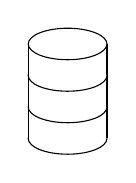
\begin{tikzpicture}[rounded corners=.5pt]
    \draw[fill=white] (.5,0) ellipse (.5cm and .2cm);  


    \draw[draw=none,fill=white] (0,0) rectangle (1,.4);
    \draw[] (0,0) -- (0,.4);
    \draw[] (1,0) -- (1,.4);    
    \draw[fill=white] (.5,.4) ellipse (.5cm and .2cm);  

    \draw[draw=none,fill=white] (0,.4) rectangle (1,.8);
    \draw[] (0,.4) -- (0,.8);
    \draw[] (1,.4) -- (1,.8);    
    \draw[fill=white] (.5,.8) ellipse (.5cm and .2cm);  


    \draw[draw=none,fill=white] (0,.8) rectangle (1,1.2);
    \draw[] (0,.8) -- (0,1.2);
    \draw[] (1,.8) -- (1,1.2);    
    \draw[fill=white] (.5,1.2) ellipse (.5cm and .2cm);  
\end{tikzpicture}
\end{document}}};
\node[secretcr] at (0,1.5) {Assignment};
\node[secretcr] at (0,1.1) {Database};
\node[secretcr] at (4,-2) {\resizebox{1cm}{!}{\documentclass[tikz]{standalone}
\begin{document}
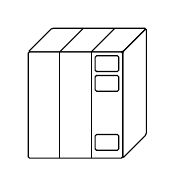
\begin{tikzpicture}[rounded corners=.5pt]
    \draw (0,0) rectangle (1.2,1.35);
    \draw (.4,0) -- (.4,1.35);
    \draw (.8,0) -- (.8,1.35);

    \draw (0,0)+(.85,1.1) rectangle ([shift={(.85, 1.1)}] .3, .2);
    \draw (0,0)+(.85,.85) rectangle ([shift={(.85, .85)}] .3, .2);
    \draw (0,0)+(.85,.1) rectangle ([shift={(.85, .1)}] .3, .2);

    \draw (1.2,0) -- (1.2,1.35) -- (1.5,1.65) -- (1.5,.3) -- cycle;

    \draw (0,1.35) -- (.3,1.65) -- (1.5,1.65) -- (1.2,1.35) -- cycle;
    \draw (.4,1.35) -- (.7,1.65);
    \draw (.8,1.35) -- (1.1,1.65);    
\end{tikzpicture}
\end{document}}};
\node[secretcr] at (4,-3) {Deploy};
\node[secretcr] at (4,-3.4) {Server};
\node[secretcr] at (4,2) {\resizebox{1cm}{!}{\documentclass[tikz]{standalone}
\begin{document}

\begin{tikzpicture}[rounded corners=.1pt]
    \draw (-.15,-.1) rectangle (.95,.5);
    \draw[fill=white] (0,0) rectangle (1,.8);
    \draw[fill=white] (0,0) -- (-.2,.1) -- (-.2,.9) -- (.8,.9) -- (1,.8) -- (0,.8) --
    cycle;
    \draw (0,.8) -- (-.2,.9);
    \draw[fill=white] (0,-.05) -- (1,-.05) -- (1,-.25) -- (0,-.25) -- cycle;
    \draw[fill=white] (0,-.05) -- (0,-.25) -- (-.2,-.15) -- (-.2,.05) -- cycle;
    \draw[rounded corners=.5pt,fill=gray] (.1,.1) rectangle  (.9,.7);
    \draw (-.2,-.25) -- (1.1,-.25) -- (1.2,-.37) -- (-.1,-.37) -- cycle;
    \draw (-.2,-.25) -- (-.2,-.3) -- (-.1,-.4) -- (-.1,-.37) -- cycle;
    \draw (-.1,-.4) rectangle (1.2,-.37);
\end{tikzpicture}
\end{document}}};
\node[secretcr] at (4,3) {Self-learner};
\draw[secretcr,->,ultra thick] (4.2,-1.4) -- (4.2,1.4);
\draw[secretcr,<-,ultra thick] (3.8,-1.4) -- (3.8,1.4);

\draw[secretcr,->,ultra thick] (-3,1.97) --(-.6,.35);%Up Left (1.8->1.97
\draw[secretcr,<-,ultra thick] (-3.1,1.72) -- (-.7,.1);

\draw[secretcr,->,ultra thick] (3,1.97) --(.6,.35);%up right
\draw[secretcr,<-,ultra thick] (3.1,1.72) -- (.7,.1);

\draw[secretcr,->,ultra thick] (3.2,-2.05) --(.8,-.43);%Down right .6 ->.6-1.7
\draw[secretcr,<-,ultra thick] (3.1,-2.25) -- (.7,-.63); %.8 -1.7 = .63
 \end{slideb}
 
 \begin{slideb}{.3}
 \end{slideb}

 \begin{slideb}{.1}
  \node[secretcr] at (-4,2) [cloud,draw, cloud puffs=10,cloud puff arc=120,
    aspect=2, inner ysep=1em,scale=.8] {};
\node[secretcr] at (-4,2) {LMS};
\node[secretcr] at (-4,-2) {\resizebox{1cm}{!}{\documentclass[tikz]{standalone}
\begin{document}

\begin{tikzpicture}[rounded corners=.1pt]
    \draw (-.15,-.1) rectangle (.95,.5);
    \draw[fill=white] (0,0) rectangle (1,.8);
    \draw[fill=white] (0,0) -- (-.2,.1) -- (-.2,.9) -- (.8,.9) -- (1,.8) -- (0,.8) --
    cycle;
    \draw (0,.8) -- (-.2,.9);
    \draw[fill=white] (0,-.05) -- (1,-.05) -- (1,-.25) -- (0,-.25) -- cycle;
    \draw[fill=white] (0,-.05) -- (0,-.25) -- (-.2,-.15) -- (-.2,.05) -- cycle;
    \draw[rounded corners=.5pt,fill=gray] (.1,.1) rectangle  (.9,.7);
    \draw (-.2,-.25) -- (1.1,-.25) -- (1.2,-.37) -- (-.1,-.37) -- cycle;
    \draw (-.2,-.25) -- (-.2,-.3) -- (-.1,-.4) -- (-.1,-.37) -- cycle;
    \draw (-.1,-.4) rectangle (1.2,-.37);
\end{tikzpicture}
\end{document}}};
\node[secretcr] at (-4,-3) {Students with LTI};
\draw[secretcr,->,ultra thick] (-4.2,-1.4) -- (-4.2,1.4);
\draw[secretcr,<-,ultra thick] (-3.8,-1.4) -- (-3.8,1.4);
\node[secretcr] at (0,0) {\resizebox{1cm}{!}{\documentclass[tikz]{standalone}
\begin{document}
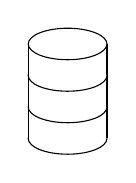
\begin{tikzpicture}[rounded corners=.5pt]
    \draw[fill=white] (.5,0) ellipse (.5cm and .2cm);  


    \draw[draw=none,fill=white] (0,0) rectangle (1,.4);
    \draw[] (0,0) -- (0,.4);
    \draw[] (1,0) -- (1,.4);    
    \draw[fill=white] (.5,.4) ellipse (.5cm and .2cm);  

    \draw[draw=none,fill=white] (0,.4) rectangle (1,.8);
    \draw[] (0,.4) -- (0,.8);
    \draw[] (1,.4) -- (1,.8);    
    \draw[fill=white] (.5,.8) ellipse (.5cm and .2cm);  


    \draw[draw=none,fill=white] (0,.8) rectangle (1,1.2);
    \draw[] (0,.8) -- (0,1.2);
    \draw[] (1,.8) -- (1,1.2);    
    \draw[fill=white] (.5,1.2) ellipse (.5cm and .2cm);  
\end{tikzpicture}
\end{document}}};
\node[secretcr] at (0,1.5) {Assignment};
\node[secretcr] at (0,1.1) {Database};
\node[secretcr] at (4,-2) {\resizebox{1cm}{!}{\documentclass[tikz]{standalone}
\begin{document}
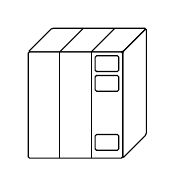
\begin{tikzpicture}[rounded corners=.5pt]
    \draw (0,0) rectangle (1.2,1.35);
    \draw (.4,0) -- (.4,1.35);
    \draw (.8,0) -- (.8,1.35);

    \draw (0,0)+(.85,1.1) rectangle ([shift={(.85, 1.1)}] .3, .2);
    \draw (0,0)+(.85,.85) rectangle ([shift={(.85, .85)}] .3, .2);
    \draw (0,0)+(.85,.1) rectangle ([shift={(.85, .1)}] .3, .2);

    \draw (1.2,0) -- (1.2,1.35) -- (1.5,1.65) -- (1.5,.3) -- cycle;

    \draw (0,1.35) -- (.3,1.65) -- (1.5,1.65) -- (1.2,1.35) -- cycle;
    \draw (.4,1.35) -- (.7,1.65);
    \draw (.8,1.35) -- (1.1,1.65);    
\end{tikzpicture}
\end{document}}};
\node[secretcr] at (4,-3) {Deploy};
\node[secretcr] at (4,-3.4) {Server};
\node[secretcr] at (4,2) {\resizebox{1cm}{!}{\documentclass[tikz]{standalone}
\begin{document}

\begin{tikzpicture}[rounded corners=.1pt]
    \draw (-.15,-.1) rectangle (.95,.5);
    \draw[fill=white] (0,0) rectangle (1,.8);
    \draw[fill=white] (0,0) -- (-.2,.1) -- (-.2,.9) -- (.8,.9) -- (1,.8) -- (0,.8) --
    cycle;
    \draw (0,.8) -- (-.2,.9);
    \draw[fill=white] (0,-.05) -- (1,-.05) -- (1,-.25) -- (0,-.25) -- cycle;
    \draw[fill=white] (0,-.05) -- (0,-.25) -- (-.2,-.15) -- (-.2,.05) -- cycle;
    \draw[rounded corners=.5pt,fill=gray] (.1,.1) rectangle  (.9,.7);
    \draw (-.2,-.25) -- (1.1,-.25) -- (1.2,-.37) -- (-.1,-.37) -- cycle;
    \draw (-.2,-.25) -- (-.2,-.3) -- (-.1,-.4) -- (-.1,-.37) -- cycle;
    \draw (-.1,-.4) rectangle (1.2,-.37);
\end{tikzpicture}
\end{document}}};
\node[secretcr] at (4,3) {Self-learner};
\draw[secretcr,->,ultra thick] (4.2,-1.4) -- (4.2,1.4);
\draw[secretcr,<-,ultra thick] (3.8,-1.4) -- (3.8,1.4);

\draw[secretcr,->,ultra thick] (-3,1.97) --(-.6,.35);%Up Left (1.8->1.97
\draw[secretcr,<-,ultra thick] (-3.1,1.72) -- (-.7,.1);

\draw[secretcr,->,ultra thick] (3,1.97) --(.6,.35);%up right
\draw[secretcr,<-,ultra thick] (3.1,1.72) -- (.7,.1);

\draw[secretcr,->,ultra thick] (3.2,-2.05) --(.8,-.43);%Down right .6 ->.6-1.7
\draw[secretcr,<-,ultra thick] (3.1,-2.25) -- (.7,-.63); %.8 -1.7 = .63
 \end{slideb}
 
 \begin{slideb}{.1}
 \end{slideb}

 \begin{slideb}{5}
  \node[secretcr] at (-4,2) [cloud,draw, cloud puffs=10,cloud puff arc=120,
    aspect=2, inner ysep=1em,scale=.8] {};
\node[secretcr] at (-4,2) {LMS};
\node[secretcr] at (-4,-2) {\resizebox{1cm}{!}{\documentclass[tikz]{standalone}
\begin{document}

\begin{tikzpicture}[rounded corners=.1pt]
    \draw (-.15,-.1) rectangle (.95,.5);
    \draw[fill=white] (0,0) rectangle (1,.8);
    \draw[fill=white] (0,0) -- (-.2,.1) -- (-.2,.9) -- (.8,.9) -- (1,.8) -- (0,.8) --
    cycle;
    \draw (0,.8) -- (-.2,.9);
    \draw[fill=white] (0,-.05) -- (1,-.05) -- (1,-.25) -- (0,-.25) -- cycle;
    \draw[fill=white] (0,-.05) -- (0,-.25) -- (-.2,-.15) -- (-.2,.05) -- cycle;
    \draw[rounded corners=.5pt,fill=gray] (.1,.1) rectangle  (.9,.7);
    \draw (-.2,-.25) -- (1.1,-.25) -- (1.2,-.37) -- (-.1,-.37) -- cycle;
    \draw (-.2,-.25) -- (-.2,-.3) -- (-.1,-.4) -- (-.1,-.37) -- cycle;
    \draw (-.1,-.4) rectangle (1.2,-.37);
\end{tikzpicture}
\end{document}}};
\node[secretcr] at (-4,-3) {Students with LTI};
\draw[secretcr,->,ultra thick] (-4.2,-1.4) -- (-4.2,1.4);
\draw[secretcr,<-,ultra thick] (-3.8,-1.4) -- (-3.8,1.4);
\node[secretcr] at (0,0) {\resizebox{1cm}{!}{\documentclass[tikz]{standalone}
\begin{document}
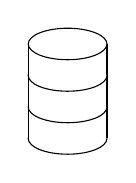
\begin{tikzpicture}[rounded corners=.5pt]
    \draw[fill=white] (.5,0) ellipse (.5cm and .2cm);  


    \draw[draw=none,fill=white] (0,0) rectangle (1,.4);
    \draw[] (0,0) -- (0,.4);
    \draw[] (1,0) -- (1,.4);    
    \draw[fill=white] (.5,.4) ellipse (.5cm and .2cm);  

    \draw[draw=none,fill=white] (0,.4) rectangle (1,.8);
    \draw[] (0,.4) -- (0,.8);
    \draw[] (1,.4) -- (1,.8);    
    \draw[fill=white] (.5,.8) ellipse (.5cm and .2cm);  


    \draw[draw=none,fill=white] (0,.8) rectangle (1,1.2);
    \draw[] (0,.8) -- (0,1.2);
    \draw[] (1,.8) -- (1,1.2);    
    \draw[fill=white] (.5,1.2) ellipse (.5cm and .2cm);  
\end{tikzpicture}
\end{document}}};
\node[secretcr] at (0,1.5) {Assignment};
\node[secretcr] at (0,1.1) {Database};
\node[secretcr] at (4,-2) {\resizebox{1cm}{!}{\documentclass[tikz]{standalone}
\begin{document}
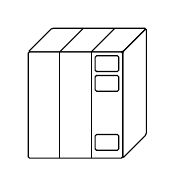
\begin{tikzpicture}[rounded corners=.5pt]
    \draw (0,0) rectangle (1.2,1.35);
    \draw (.4,0) -- (.4,1.35);
    \draw (.8,0) -- (.8,1.35);

    \draw (0,0)+(.85,1.1) rectangle ([shift={(.85, 1.1)}] .3, .2);
    \draw (0,0)+(.85,.85) rectangle ([shift={(.85, .85)}] .3, .2);
    \draw (0,0)+(.85,.1) rectangle ([shift={(.85, .1)}] .3, .2);

    \draw (1.2,0) -- (1.2,1.35) -- (1.5,1.65) -- (1.5,.3) -- cycle;

    \draw (0,1.35) -- (.3,1.65) -- (1.5,1.65) -- (1.2,1.35) -- cycle;
    \draw (.4,1.35) -- (.7,1.65);
    \draw (.8,1.35) -- (1.1,1.65);    
\end{tikzpicture}
\end{document}}};
\node[secretcr] at (4,-3) {Deploy};
\node[secretcr] at (4,-3.4) {Server};
\node[secretcr] at (4,2) {\resizebox{1cm}{!}{\documentclass[tikz]{standalone}
\begin{document}

\begin{tikzpicture}[rounded corners=.1pt]
    \draw (-.15,-.1) rectangle (.95,.5);
    \draw[fill=white] (0,0) rectangle (1,.8);
    \draw[fill=white] (0,0) -- (-.2,.1) -- (-.2,.9) -- (.8,.9) -- (1,.8) -- (0,.8) --
    cycle;
    \draw (0,.8) -- (-.2,.9);
    \draw[fill=white] (0,-.05) -- (1,-.05) -- (1,-.25) -- (0,-.25) -- cycle;
    \draw[fill=white] (0,-.05) -- (0,-.25) -- (-.2,-.15) -- (-.2,.05) -- cycle;
    \draw[rounded corners=.5pt,fill=gray] (.1,.1) rectangle  (.9,.7);
    \draw (-.2,-.25) -- (1.1,-.25) -- (1.2,-.37) -- (-.1,-.37) -- cycle;
    \draw (-.2,-.25) -- (-.2,-.3) -- (-.1,-.4) -- (-.1,-.37) -- cycle;
    \draw (-.1,-.4) rectangle (1.2,-.37);
\end{tikzpicture}
\end{document}}};
\node[secretcr] at (4,3) {Self-learner};
\draw[secretcr,->,ultra thick] (4.2,-1.4) -- (4.2,1.4);
\draw[secretcr,<-,ultra thick] (3.8,-1.4) -- (3.8,1.4);

\draw[secretcr,->,ultra thick] (-3,1.97) --(-.6,.35);%Up Left (1.8->1.97
\draw[secretcr,<-,ultra thick] (-3.1,1.72) -- (-.7,.1);

\draw[secretcr,->,ultra thick] (3,1.97) --(.6,.35);%up right
\draw[secretcr,<-,ultra thick] (3.1,1.72) -- (.7,.1);

\draw[secretcr,->,ultra thick] (3.2,-2.05) --(.8,-.43);%Down right .6 ->.6-1.7
\draw[secretcr,<-,ultra thick] (3.1,-2.25) -- (.7,-.63); %.8 -1.7 = .63
 \end{slideb}
 

\foreach \i in {0,.05,...,1} {
\begin{slideb}{.1}
  \node[secretcr] at (-4,2) [cloud,draw, cloud puffs=10,cloud puff arc=120,
    aspect=2, inner ysep=1em,scale=.8] {};
\node[secretcr] at (-4,2) {LMS};
\node[secretcr] at (-4,-2) {\resizebox{1cm}{!}{\documentclass[tikz]{standalone}
\begin{document}

\begin{tikzpicture}[rounded corners=.1pt]
    \draw (-.15,-.1) rectangle (.95,.5);
    \draw[fill=white] (0,0) rectangle (1,.8);
    \draw[fill=white] (0,0) -- (-.2,.1) -- (-.2,.9) -- (.8,.9) -- (1,.8) -- (0,.8) --
    cycle;
    \draw (0,.8) -- (-.2,.9);
    \draw[fill=white] (0,-.05) -- (1,-.05) -- (1,-.25) -- (0,-.25) -- cycle;
    \draw[fill=white] (0,-.05) -- (0,-.25) -- (-.2,-.15) -- (-.2,.05) -- cycle;
    \draw[rounded corners=.5pt,fill=gray] (.1,.1) rectangle  (.9,.7);
    \draw (-.2,-.25) -- (1.1,-.25) -- (1.2,-.37) -- (-.1,-.37) -- cycle;
    \draw (-.2,-.25) -- (-.2,-.3) -- (-.1,-.4) -- (-.1,-.37) -- cycle;
    \draw (-.1,-.4) rectangle (1.2,-.37);
\end{tikzpicture}
\end{document}}};
\node[secretcr] at (-4,-3) {Students with LTI};
\draw[secretcr,->,ultra thick] (-4.2,-1.4) -- (-4.2,1.4);
\draw[secretcr,<-,ultra thick] (-3.8,-1.4) -- (-3.8,1.4);
\node[secretcr] at (0,0) {\resizebox{1cm}{!}{\documentclass[tikz]{standalone}
\begin{document}
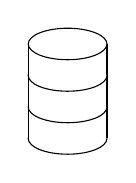
\begin{tikzpicture}[rounded corners=.5pt]
    \draw[fill=white] (.5,0) ellipse (.5cm and .2cm);  


    \draw[draw=none,fill=white] (0,0) rectangle (1,.4);
    \draw[] (0,0) -- (0,.4);
    \draw[] (1,0) -- (1,.4);    
    \draw[fill=white] (.5,.4) ellipse (.5cm and .2cm);  

    \draw[draw=none,fill=white] (0,.4) rectangle (1,.8);
    \draw[] (0,.4) -- (0,.8);
    \draw[] (1,.4) -- (1,.8);    
    \draw[fill=white] (.5,.8) ellipse (.5cm and .2cm);  


    \draw[draw=none,fill=white] (0,.8) rectangle (1,1.2);
    \draw[] (0,.8) -- (0,1.2);
    \draw[] (1,.8) -- (1,1.2);    
    \draw[fill=white] (.5,1.2) ellipse (.5cm and .2cm);  
\end{tikzpicture}
\end{document}}};
\node[secretcr] at (0,1.5) {Assignment};
\node[secretcr] at (0,1.1) {Database};
\node[secretcr] at (4,-2) {\resizebox{1cm}{!}{\documentclass[tikz]{standalone}
\begin{document}
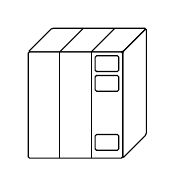
\begin{tikzpicture}[rounded corners=.5pt]
    \draw (0,0) rectangle (1.2,1.35);
    \draw (.4,0) -- (.4,1.35);
    \draw (.8,0) -- (.8,1.35);

    \draw (0,0)+(.85,1.1) rectangle ([shift={(.85, 1.1)}] .3, .2);
    \draw (0,0)+(.85,.85) rectangle ([shift={(.85, .85)}] .3, .2);
    \draw (0,0)+(.85,.1) rectangle ([shift={(.85, .1)}] .3, .2);

    \draw (1.2,0) -- (1.2,1.35) -- (1.5,1.65) -- (1.5,.3) -- cycle;

    \draw (0,1.35) -- (.3,1.65) -- (1.5,1.65) -- (1.2,1.35) -- cycle;
    \draw (.4,1.35) -- (.7,1.65);
    \draw (.8,1.35) -- (1.1,1.65);    
\end{tikzpicture}
\end{document}}};
\node[secretcr] at (4,-3) {Deploy};
\node[secretcr] at (4,-3.4) {Server};
\node[secretcr] at (4,2) {\resizebox{1cm}{!}{\documentclass[tikz]{standalone}
\begin{document}

\begin{tikzpicture}[rounded corners=.1pt]
    \draw (-.15,-.1) rectangle (.95,.5);
    \draw[fill=white] (0,0) rectangle (1,.8);
    \draw[fill=white] (0,0) -- (-.2,.1) -- (-.2,.9) -- (.8,.9) -- (1,.8) -- (0,.8) --
    cycle;
    \draw (0,.8) -- (-.2,.9);
    \draw[fill=white] (0,-.05) -- (1,-.05) -- (1,-.25) -- (0,-.25) -- cycle;
    \draw[fill=white] (0,-.05) -- (0,-.25) -- (-.2,-.15) -- (-.2,.05) -- cycle;
    \draw[rounded corners=.5pt,fill=gray] (.1,.1) rectangle  (.9,.7);
    \draw (-.2,-.25) -- (1.1,-.25) -- (1.2,-.37) -- (-.1,-.37) -- cycle;
    \draw (-.2,-.25) -- (-.2,-.3) -- (-.1,-.4) -- (-.1,-.37) -- cycle;
    \draw (-.1,-.4) rectangle (1.2,-.37);
\end{tikzpicture}
\end{document}}};
\node[secretcr] at (4,3) {Self-learner};
\draw[secretcr,->,ultra thick] (4.2,-1.4) -- (4.2,1.4);
\draw[secretcr,<-,ultra thick] (3.8,-1.4) -- (3.8,1.4);

\draw[secretcr,->,ultra thick] (-3,1.97) --(-.6,.35);%Up Left (1.8->1.97
\draw[secretcr,<-,ultra thick] (-3.1,1.72) -- (-.7,.1);

\draw[secretcr,->,ultra thick] (3,1.97) --(.6,.35);%up right
\draw[secretcr,<-,ultra thick] (3.1,1.72) -- (.7,.1);

\draw[secretcr,->,ultra thick] (3.2,-2.05) --(.8,-.43);%Down right .6 ->.6-1.7
\draw[secretcr,<-,ultra thick] (3.1,-2.25) -- (.7,-.63); %.8 -1.7 = .63
  \draw[fill=black,opacity={\i}] (-10,-10) rectangle (10,10);
  \node[opacity=\i] at (0,0) {
    \includegraphics[width=.5\textwidth]{mx.png}};
\end{slideb}
}

\begin{slideb}{1}
  \node[opacity=1] at (0,0) {
    \includegraphics[width=.5\textwidth]{mx.png}};
\end{slideb}


\foreach \i in {1,.95,...,0} {
  \begin{slideb}{.1}
    \node[opacity=1] at (0,0) {
      \includegraphics[width=.5\textwidth]{mx.png}};
    \node[secretcr] at (0,-4) {\resizebox{6in}{.2in}{MODULUS IS COMING}};
    \draw[fill=black,opacity=\i] (-4in,-2in) rectangle (4in,-1.4in);
  \end{slideb}
  }


  \begin{slideb}{3}
    \node[opacity=1] at (0,0) {
      \includegraphics[width=.5\textwidth]{mx.png}};
    \node[secretcr] at (0,-4) {\resizebox{6in}{.2in}{MODULUS IS COMING}};
  \end{slideb}
  


\end{document}
